\documentclass[twoside]{article}
\usepackage[a4paper]{geometry}
\geometry{verbose,tmargin=2.5cm,bmargin=2cm,lmargin=2cm,rmargin=2cm}
\usepackage{fancyhdr}
\pagestyle{fancy}

% nastavení pisma a češtiny
\usepackage{lmodern}
\usepackage[T1]{fontenc}
\usepackage[utf8]{inputenc}
\usepackage[czech]{babel}

% odkazy
\usepackage{url}

\usepackage{float}
% vícesloupcové tabulky
\usepackage{multirow}
\usepackage{amssymb}
\usepackage{bbold}
\usepackage{amsmath}
\usepackage{commath}

% vnořené popisky obrázků
\usepackage{subcaption}

% automatická konverze EPS 
\usepackage{graphicx} 
\usepackage{epstopdf}
\epstopdfsetup{update}

\graphicspath{{./images}}

% odkazy a záložky
\usepackage[unicode=true, bookmarks=true,bookmarksnumbered=true,
bookmarksopen=false, breaklinks=false,pdfborder={0 0 0},
pdfpagemode=UseNone,backref=false,colorlinks=true] {hyperref}

% Poznámky při překladu
\usepackage{xkeyval}	% Inline todonotes
\usepackage[textsize = footnotesize]{todonotes}
\presetkeys{todonotes}{inline}{}

% Zacni sekci slovem ukol
\renewcommand{\thesection}{Úkol \arabic{section}}
% enumerate zacina s pismenem
\renewcommand{\theenumi}{\alph{enumi}}

% smaz aktualni page layout
\fancyhf{}
% zahlavi
\usepackage{titling}
\fancyhf[HC]{\thetitle}
\fancyhf[HLE,HRO]{\theauthor}
\fancyhf[HRE,HLO]{\today}
 %zapati
\fancyhf[FLE,FRO]{\thepage}

% údaje o autorovi
\title{Automatické řízení: DÚ 0 - opakování předmětu SAS}

\author{Vojtěch Michal}
\date{\today}

\begin{document}

\maketitle

% ---------------------------------
% ---------------------------------
% název sekce je generován automaticky jako: Úkol X
\section{Ustálená odezva}
\label{sec:ukol1}

\subsection{~}
\label{sec:ukol1:1}
Nalezněte statické zesílení K systému popsaného níže uvedeným přenosem.
\begin{equation}
	G(s) = \frac{-0.2s+5}{(s+3)(s+2)(s+1)}
\end{equation}
\textbf{Řešení:} Statické zesílení je konečná hodnota odezvy na jednotkový skok $w(t)$. Podle věty o konečné hodnotě
\begin{equation}
	\lim_{t \to \infty}w(t) = \lim_{s \to 0}sW(s)
\end{equation}
pro statické zesílení K plyne:
\begin{equation}
	\label{eq:dcgain}
	K = \lim_{t \to \infty}w(t) = \lim_{s \to 0}{\underbrace{sW(s)}_{=G(s)}} = \frac{0+5}{(0+3)(0+2)(0+1)} = \frac{5}{6}.
\end{equation}
Statické zesílení zadaného vnějšího modelu je $K = \frac{5}{6}$.

\subsection{~}
Zjistěte ustálenou hodnotu odezvy na vstup $u (t) = 5$. Své tvrzení odvoďte. \\
\textbf{Řešení:} Nejdříve je potřeba ověřit, že nějaká ustálená hodnota bude existovat. Zřejmě ano, protože přenosová funkce má všechny póly
v levé polorovině s. Využijeme linearity systému a Laplaceovy transformace. Protože $u(t) = 5\cdot \mathbb{1}(t)$, platí pro výstup $y(t)$:
\begin{equation}
	y(t) = \mathcal{L}^{-1}\{G(s) \cdot \mathcal{L}\{u(t)\}\} = 5~\mathcal{L}^{-1}\{\underbrace{G(s) \cdot \mathcal{L}\{\mathbb{1}(t)\}}_{= \frac{1}{s}G(s)=W(s)}\}
	= 5 w(t) \longrightarrow_{t \to \infty} 5 K.
\end{equation}
Se znalostí statického zesílení podle \eqref{eq:dcgain} je vidět, že se výstup ustálí na hodnotě $y(t)=\frac{25}{6}$.


\subsection{~}
\label{sec:ukol1:3}
Jaká bude ustálená hodnota odezvy na Dirakův impulz? \\
\textbf{Řešení:} Odezvy na jednotkový skok $w(t)$ a na Diracův impuls $h(t)$ spojuje vztah $w(t) = \int h(t)$. Z \ref{sec:ukol1:1} již víme, že $w(t)$ se ustálí
na konstantní hodnotě $K$, její derivace $h(t)$ tedy po ustálení musí být nulová. Pro ustálenou hodnotu impulsové odezvy tedy platí $\lim_{t \to \infty} h(t) = 0$.

% ---------------------------------
\section{Laplaceova transformace}
\label{sec:ukol2}
\subsection{~}
Pomocí Laplaceovy transformace vyřešte následující soustavu diferenciálních rovnic
\begin{equation*}
	\begin{split}
		\dot{x_1} &= - 6x_1 (t) + 26x_2 (t), \\
		\dot{x_2} &= - 0.5 x_1(t),
	\end{split}
\end{equation*}
za počátečních podmínek
\begin{equation*}
	\vec{x}_0 = \begin{bmatrix}
		2 \\
		0
	  \end{bmatrix}.
\end{equation*} \\
\textbf{Řešení:} Převeďme soustavu do maticového tvaru
\begin{equation*}
	\dot{\vec{x}}(t) = \underbrace{\begin{bmatrix}
		-6 & 26 \\
		-0.5 & 0
	\end{bmatrix}}_{A} \vec{x}(t)
\end{equation*}
a transformujme Laplaceovou transformací. Nechť $\mathcal{L}\{\vec{t}(t)\} = X(s)$, poté
\begin{equation}
	\label{eq:laplace-boi}
	s\vec{X}(s) - \vec{x_0} = A\vec{X}(s) \Rightarrow \vec{X}(s) = (sI-A)^{-1}\vec{x_0}.
\end{equation}
Po dosazení zadaných hodnot do rovnice \eqref{eq:laplace-boi} získám
\begin{equation*}
	\vec{X}(s) = \underbrace{\begin{bmatrix}
		s + 6 & -26 \\
		0.5 & s
	\end{bmatrix}^{-1}}_{=(sI - A)} \begin{bmatrix}
		2 \\
		0
	\end{bmatrix} = \underbrace{\frac{1}{s(s+6) + 13}}_{=\text{det}^{-1}(sI - A)} \underbrace{\begin{bmatrix}
		s & 26 \\
		-0.5 & s + 6
	\end{bmatrix}}_{\text{adj}(sI - A)} \begin{bmatrix}
		2 \\
		0
	\end{bmatrix} = \frac{1}{s^2 + 6s + 13} \begin{bmatrix}
		2s \\
		-1
	\end{bmatrix}.
\end{equation*}
Pro obrazy funkcí $x_1(t)$, $x_2(t)$ po složkách platí
\begin{equation*}
	\begin{split}
		x_1(s) &= \frac{2s}{s^2 + 6s + 13} \\
		x_2(s) &= \frac{-1}{s^2 + 6s + 13}
	\end{split}
\end{equation*}
a obě identity invertujeme. Jmenovatel má kořeny $s_{1,2} = -3 \pm 2i$, označme $\sigma = -3$, $\omega = 2$. Očekávám, že řešení bude složeno 
z kvazipolynomů s $\text{exp}(\sigma t)$, $\text{sin}(\omega t)$ a $\text{cos}(\omega t)$.
\begin{equation*}
	\begin{split}
		x_1(t) &= \mathcal{L}^{-1}\{\frac{2s}{(s+3)^2 + 4}\} = \mathcal{L}^{-1}\{\frac{2(s - \sigma)}{(s-\sigma)^2 + \omega^2}\} + \mathcal{L}^{-1}\{\frac{2\sigma}{(s-\sigma)^2 + \omega^2}\} = 
		2 e^{\sigma t} \text{cos}(\omega t) + 2 \frac{\sigma}{\omega} e^{\sigma t} \text{sin}(\omega t),\\
		x_2(t) &= \mathcal{L}^{-1}\{\frac{-1}{(s+3)^2 + 4}\} = \mathcal{L}^{-1}\{\frac{-0.5 \omega}{(s-\sigma)^2 + \omega^2}\} = -\frac{1}{2} e^{\sigma t} \text{sin}(\omega t).
	\end{split}
\end{equation*}
Po vyčíslení obdržíme
\begin{equation*}
	\begin{split}
		x_1(t) &= e^{-3t}(2\text{cos}(2t) -3 \text{sin}(2t)), \\
		x_2(t) &= -0.5 e^{-3t}\text{sin}(2t).
	\end{split}
\end{equation*}

\subsection{~}
\begin{figure}[htbp]
	\includegraphics{solution22.eps}
	\caption{Časové průběhy řešení úlohy 2.2}
	\label{fig:reseni22}
\end{figure}
Vykreslete průběhy nalezených funkcí v Matlabu. \\
\textbf{Řešení} je vykresleno na obrázku \ref{fig:reseni22}.

\section{Linearizace}
\label{sec:ukol3}
Je zadaný systém
\begin{equation}
	\begin{split}
		\dot{x_1} &= f_1(\vec{x}, u) = x_2 \\
		\dot{x_2} &= f_2(\vec{x}, u) = -2 \text{sin}(x_1) - 0.1x_2 +u \\
		y &= x_1
	\end{split}
	\label{eq:nelinearni}
\end{equation}

\subsection{~}
Nalezněte rovnovážný pracovní bod systému $P = \begin{bmatrix} x_{1p}, x_{2p}, y_p \end{bmatrix}$ pro $u_p (t) = 2$. \\
\textbf{Řešení:} V rovnovážném bodě jsou derivace stavových proměnných nulové, tedy $\dot{\vec{x}} = \vec{o}$.
Využijeme této podmínky pro úpravu \eqref{eq:nelinearni} a nalezení $P$:
\begin{equation}
	\begin{split}
		x_{2p} &= 0\\
		0 = -2 \text{sin}(x_{1p}) - \underbrace{0.1x_{2p}}_{=0} +u_p \Rightarrow \text{sin}(x_{1p}) &= 1 \\
		y_p &= x_{1p}
	\end{split}
\end{equation}
Periodicita funkce sin ve druhé rovnici způsobuje, že existuje spočené nekonečno různých pracovních bodů 
$\mathcal{P} = \{\begin{bmatrix} k\pi+\frac{\pi}{2} & 0 & k\pi+\frac{\pi}{2} \end{bmatrix} \mid\ k \in \mathbb{Z} \}$.
Díky periodicitě nelinearity systému se chování v dílčích pracovních bodech liší pouze konstantním posunem výstupu. Stačí proto linearizovat pro jeden bod, na ostatní lze snadno převádět.
Přirozená volba je vzít $x_{1p} \in \left[-\pi,\pi \right)$ proto budu linearizovat v bodě 
\begin{equation*}
	P = \begin{bmatrix} \frac{\pi}{2}, 0, \frac{\pi}{2} \end{bmatrix}.
\end{equation*}

\subsection{~}
Linearizujte systém v nalezeném pracovním bodě $P$.\\
\textbf{Řešení:} Našim cílem je nalézt matice $A$, $B$, $C$, $D$ popisující lineární systém. Linearizovat stačí funkci $f_2(\vec{x}, u)$; funkce $f_1$ i výstupní
rovnice jsou lineární. Z pohledu na soustavu jiště platí
\begin{equation*}
	D = \begin{bmatrix}
		0
	\end{bmatrix}, ~~~~~~~~~ C = \begin{bmatrix}
		1 & 0
	\end{bmatrix} ~~~~a ~~~ B = \begin{bmatrix}
		0 \\ 1
	\end{bmatrix}.
\end{equation*}
Matice $A$ bude Jacobiho matice pro funkci $f(\vec{x}, u) = (f_1, f_2)$ vyčíslená v bodě $P$.
\begin{equation*}
	A = \begin{bmatrix}
		\frac{\partial f_1}{\partial x_1} & \frac{\partial f_1}{\partial x_2} \\ 
		\frac{\partial f_2}{\partial x_1} & \frac{\partial f_2}{\partial x_2}
	\end{bmatrix}_P = \begin{bmatrix}
		0 & 1 \\
		-2\text{cos}(x_{1p}) & -0.1
	\end{bmatrix} = \begin{bmatrix}
		0 & 1 \\
		0 & -0.1
	\end{bmatrix}
\end{equation*}
Lineární aproximaci zapíšeme v odchylkovém tvaru (použijeme značení $\Delta u = u - u_p$, podobně pro $\vec{x}$ a y).
\begin{equation*}
	\begin{split}
		\Delta \dot{\vec{x}} &= A \Delta\vec{x} + B \Delta u \\
		\Delta y &= C \Delta\vec{x} + D \Delta u
	\end{split}
\end{equation*}

\

\subsection{~}
Namodelujte v Simulinku nelineární systém současně s linearizovaným. Porovnejte odezvy obou systémů
na skoky $u(t) = 1$ a $u(t) = 2.001$. \\
\textbf{Řešení:} Časové průběhy jsou na obrázku \ref{fig:linearizace}. Lineární aproximace byla provedena pro vstup $u(t) = 2$ a je tedy očekávatelné, že se pro vstup $u(t) = 1$
časové průběhy velmi rychle oddělí kvůli velké chybě způsobené zanedbáním vlivu členů vyšších řádů v Taylorově rozvoji funkce $f$.
Výstup lineárního systému diverguje, zatímco nelineární osciluje. Průběhy pro $u(t) = 2$ jsou podobnější, mají stejný typ (oba divergují k nekonečnu po exponenciále),
lineární aproximace roste mnohem pomaleji.
\begin{figure}[htbp]
    \centering % <-- added
\begin{subfigure}{0.45\textwidth}
  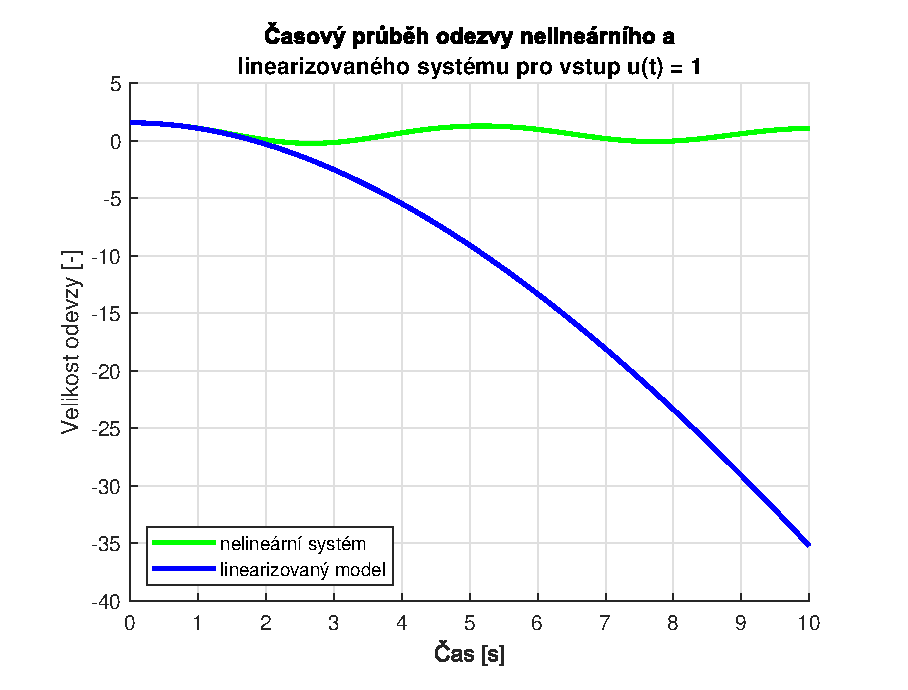
\includegraphics[width=\linewidth]{graph33_vstup1.eps}
  \caption{Simulace pro vstup $u(t) = 1$}
\end{subfigure}\hfil % <-- added
\begin{subfigure}{0.45\textwidth}
	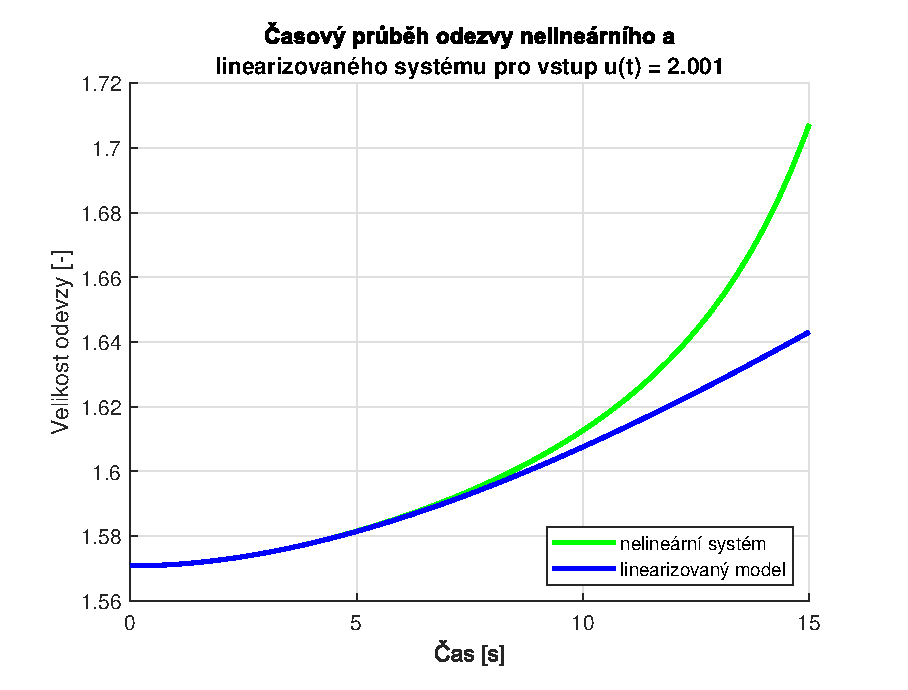
\includegraphics[width=\linewidth]{graph33_vstup2.eps}
	\caption{Simulace pro vstup $u(t) = 2.001$}
\end{subfigure}
\caption{Simulace odezev nelineárního a linearizovaného systému na různé vstupy}
\label{fig:linearizace}
\end{figure}

\section{Asymptotické frekvenční charakteristiky}
\label{sec:ukol4}

\subsection{~}
Pro následující systém nakreslete asymptotickou frekvenční charakteristiku.
\begin{equation}
	G_1(s) = \frac{s-1}{(s+10)(s-10)(s+80)}
\end{equation}
\textbf{Řešení:} Přenos nejprve upravím do podoby vhodné pro vyšetřování frekvenční charakteristiky.
\begin{equation*}
	G_1(s) = \frac{s-1}{8000(\frac{s}{10}+1)(\frac{s}{10}-1)(\frac{s}{80}+1)} = \frac{1}{8000} \frac{1-\frac{s}{\omega_1}}{(1+\frac{s}{\omega_2})(1-\frac{s}{\omega_2})(1+\frac{s}{\omega_3})}
\end{equation*}
Významné hodnoty tak jsou
\begin{itemize}
	\item nula na frekvenci $\omega_1 = 1 \text{ rad.s}^{-1}$, přispěje rostoucí amplitudou $+20$dB/dek a klesající fází,
	\item dvojnásobný pól na frekvenci $\omega_2 = 10 \text{ rad.s}^{-1}$, přispěje klesající amplitudou $-40$dB/dek, fáze konstantní,
	\item pól na $\omega_3 = 80 \text{ rad.s}^{-1}$, přispěje klesající amplitudou $-40$dB/dek a klesající fází,
	\item skalární konstanta, přispěje konstantní fází a amplitudou $20 \text{ log }\frac{1}{8000} = -78$ dB.
\end{itemize}
Výsledná frekvenční i amplitudová charakteristika se bude skládat z příspěvků od dílčích kořenových činitelů v čitateli i jmenovateli a je vidět na obrázku \ref{fig:frekchar_bode}.
\begin{figure}[htbp]
    \centering % <-- added
	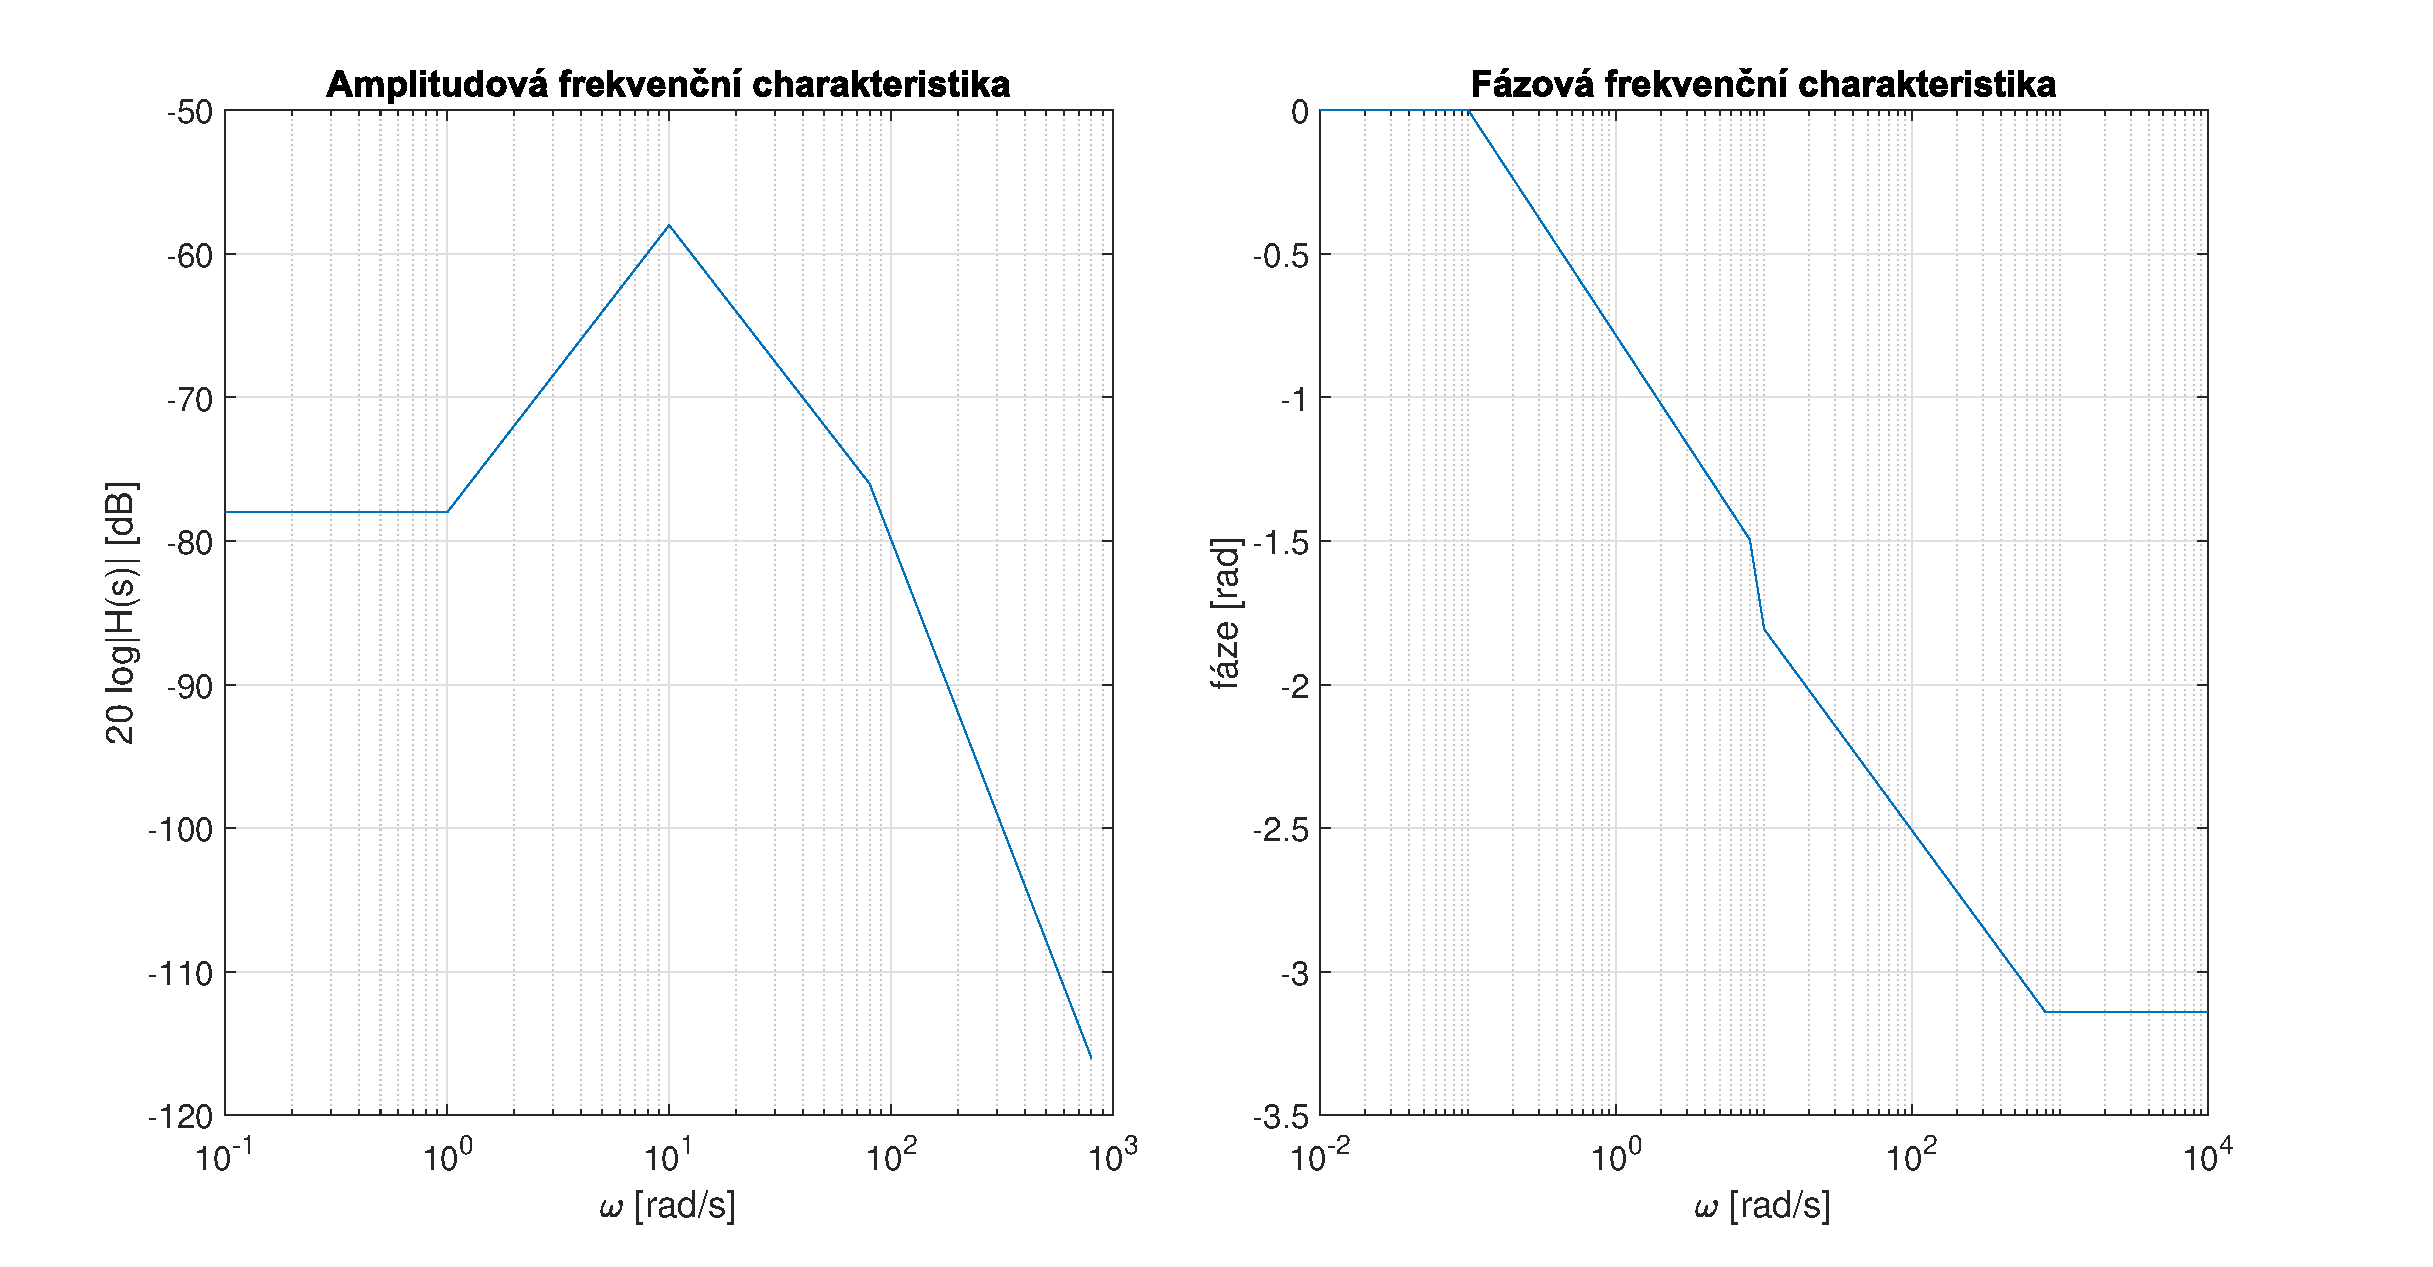
\includegraphics[width=\linewidth]{frekchar.eps}
\caption{Asymptotická frekvenční charakteristika systému z úlohy 4.1}
\label{fig:frekchar_bode}
\end{figure}

\subsection{~}

Pro asymptotickou frekvenční charakteristiku na obrázku 2 v zadání (nepovedlo se vykopírovat v obstojné kvalitě)
sestavte rovnici odpovídajícího systému s nejnižším možným počtem pólů. \\
\textbf{Řešení:} Významné body charakteristiky jsou
\begin{itemize}
	\item jednoduchý pól na $\omega_1 = 10^{-3}~\text{rad.s}^{-1}$, fáze klesá
	\item jednoduchá nula na $\omega_2 = 10^{-1}~\text{rad.s}^{-1}$, fáze klesá
	\item jednoduchá nula na $\omega_3 = 10~\text{rad.s}^{-1}$, fáze roste
	\item jednoduchý pól na $\omega_4 = 10^3~\text{rad.s}^{-1}$, fáze klesá
\end{itemize}
dále pro DC signál ($s = 0$) je zesílení 0dB, takže přenosová funkce nebude obsahovat skalární činitele.
Na základě amplitudové charakteristiky očekáváme přenosovou funkci tvaru
\begin{equation*}
	H(s) = \pm \frac{(1 \pm \frac{s}{\omega_2})(1 \pm \frac{s}{\omega_3})}{(1 \pm \frac{s}{\omega_1})(1 \pm \frac{s}{\omega_4})},
\end{equation*}
což lze odvodit z typu zalomení asymptotické amplitudové charakteristiky na konkrétních frekvencích. Pakliže se charakteristika
zalamuje dolů (směrem k - $\infty$ dB), poté je na dané frekvenci pól. Zalomení směrem nahoru (směrem k 0 dB) způsobuje nula.
O rozložení znamének plus a mínus rozhodneme na základě fázové charakteristiky. Pro činitel typu $(1 + \frac{s}{\omega})$ je fáze
nejprve konstantní a následně začne dekádu před $\omega$ s rychlostí 45° na dekádu klesat pro pól a růst pro nulu.
Na frekvenci $\omega_2$ je nula, ale fáze stále klesá. Příslušný člen tedy musí být $(1 - \frac{s}{\omega_2})$.
Ostatní činitele obsahují plus. Start s fází 180° vyžaduje záporné znaménko před celým zlomkem. Výsledný hledaný přenos je
\begin{equation*}
	H(s) = - \frac{(1-\frac{s}{0.1})(1 +\frac{s}{10})}{(1+\frac{s}{0.001})(1 + \frac{s}{1000})}.
\end{equation*}

\section{ Převod do přenosového popisu}
\label{sec:ukol5}
Převeďte následující systém do přenosového popisu. Napište postup, kterým jste k výsledku dospěli, a vybrané mezivýsledky.

\begin{equation*}
	\dot{\vec{x}} = \begin{bmatrix}
		-4 & 2 & 0 & 0 \\
		-6 & 4 & 0 & 0 \\
		-3 & 3 & 2 & -2 \\
		-9 & 9 & 2 & -3
	\end{bmatrix} \vec{x} + \begin{bmatrix}
		1 \\
		0.5 \\
	0 \\
	-1
\end{bmatrix} u ~~~~~~~~~~~
y = \begin{bmatrix}
	4 & 0 & 0 & 0
\end{bmatrix} \vec{x}
\end{equation*} \\
\textbf{Řešení:} Odvoďme maticový vzoreček pomocí stavové a výstupní rovnice a Laplaceovy transformace:
\begin{equation*}
	\begin{split}
		sX(s) &= AX(s) + B U(s) \\
		(sI - A) X(s) &= BU(s) \\
		X(s) &= (sI - A)^{-1} B U(s) \\
		Y(s) &= C \underbrace{(sI - A)^{-1} B U(s)}_{=X(s)}.
	\end{split}
\end{equation*}
Odvození je zjednodušené o to, že matice D je nulová. Přenos systému pomocí matic A, B, C poté má tvar
\begin{equation*}
	H(s) = \frac{Y(s)}{U(s)} = C(sI-A)^{-1} B.
\end{equation*}
Pro zadané matice vrátí Matlab numerické řešení
\begin{equation*}
	H(s) = \frac{4 s^3 - 12 s^2 - 16s + 48}{s^4 - 8 s^2 + 16} = \frac{(s-3)(s-2)(s+2)}{(s-2)^2(s+2)^2}.
\end{equation*}
Dává toto řešení smysl? Ve jmenovateli bychom měli mít výraz $ \det(sI - A)$, což je skutečně polynom čtvrtého
řádu v s. Dále je $D = 0$, takže by přenos měl být striktně ryzí a to je též splněno. Podobné řešení je očekávatelné,
pokud se po cestě nepokrátí činitele $(s+2)(s-2)$. Poté by byl přenos systému v principu stejný, avšak systém by obsahoval skrytý mód.

\section{Stabilita}
\label{sec:ukol6}
Rozhodněte o stabilitě systému. Výsledek zdůvodněte. \\
\begin{equation*}
	\centering
	\dot{\vec{x}} = \begin{bmatrix}
		1 & 0 & 0 \\
		2 & -2 & -2 \\
		1 & 2 & 0
	\end{bmatrix} \vec{x} + \begin{bmatrix}
		1 \\
		-1 \\
		1
\end{bmatrix} u ~~~~~~~~~~~
y = \begin{bmatrix}
	1 & 0 & -1
\end{bmatrix} \vec{x}
\end{equation*} \\
\textbf{Řešení:} Pro rozhodnutí o stabilitě ze stavového popisu lze vyšetřit znaménko vlastních čísel matice systému A.
Stabilní bude systém tehdy, když vlastní čísla budou mít zápornou reálnou část. Toto platí proto, že při převodu
stavového popisu na vnější se do jmenovatele přenosu dostane výraz $\det(sI - A)$. To je polynom v s, jeho kořeny
jsou vlastní čísla matice A, která se tak stávají póly přenosové funkce (předpokládejme, že se v přenosové funkci žádné kořenové činitele nepokrátí).

Pro zadanou matici mají vlastní čísla hodnotu $1$ a $ -1 \pm 1.73 i$. Kritérium stability tedy není splněno a systém \textbf{není stabilní} 


\section{Diskretizace}
\label{sec:ukol7}
Následující systém převeďte do diskrétního popisu, můžete využít např. metodu \textit{zero order hold}.
\begin{equation}
	G(s) = \frac{s-3}{(s+1)(s+7)}
\end{equation}

\textbf{Řešení:} Vhodný vzorkovací krok pro diskretizaci systému je alespoň o řád menší než nejmenší časová konstanta v systému.
V našem případě je nejmenší časová konstanta $\tau = \frac{1}{7}$ s, vhodný diskretičaní krok je proto například $T_1 = 10$ ms, nevhodný $T_2 = 100$ ms.
Diskretizací systému $G(s)$ se vzrokovacími frekvencemi $T_1$, $T_2$ vznikají přenosy
\begin{equation*}
	G_1(z) = \frac{0.009463z - 0.009752}{z^2 - 1.922z+0.9231} ~~~~~~\text{a}~~~~~~ G_2(z) = \frac{0.05642z - 0.07695}{z^2 - 1.401z+0.4493}.
\end{equation*}

Na obrázku \ref{fig:diskretizace} jsou pro porovnání vykresleny odezvy spojitého systému a obou diskretizací na vstupní pilový signál s frekvencí 1 hertz.
Byla použita nízká frekvence vstupu, aby obě diskretizace měly alespoň u prvních pěti harmonických dodržený vzorkovací teorém.
Diskretizace provedená s vhodným vzorkovacím krokem $T_1$ se velice věrně drží referenčního výstupu generovaného spojitým systémem.
Výstup diskretizace s nevhodným krokem $T_2$ je na první pohled odlišný. Jednak je na tvaru odezvy patrná nízká vzorkovací frekvence (časový průběh je schodovitý),
jednak se akumuluje chyba a odezva diskretizace je posunutá od odezvy spojitého systému. 
\begin{figure}[htbp]
	\centering
	\begin{subfigure}{0.45\textwidth}	
		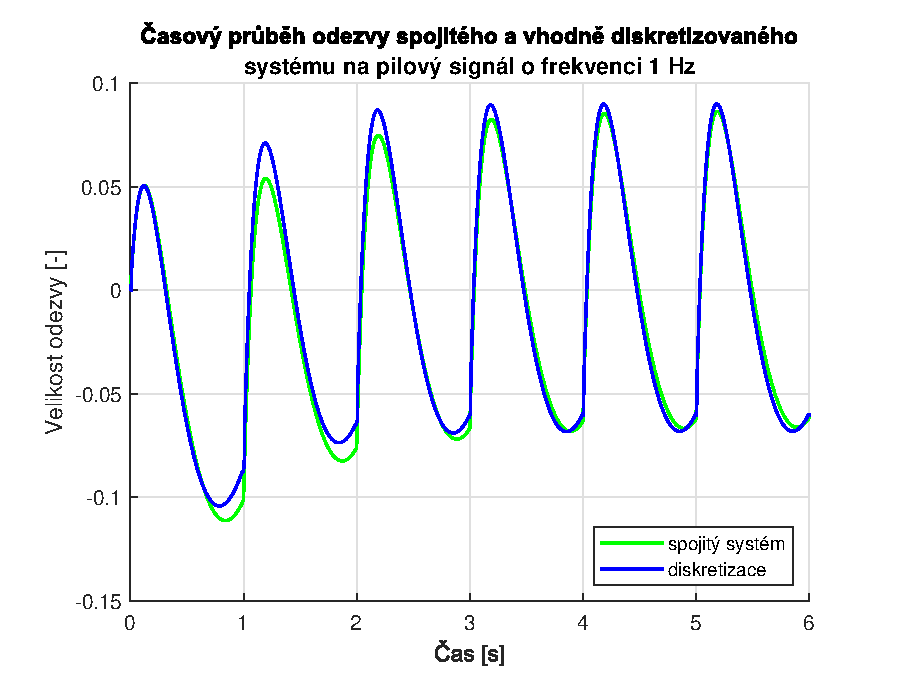
\includegraphics[width=\linewidth]{diskretizace-good.eps}
		\caption{Vhodná diskretizace s krokem $T_1 = 10$ ms}
	\end{subfigure}
	\begin{subfigure}{0.45\textwidth}
		\centering
		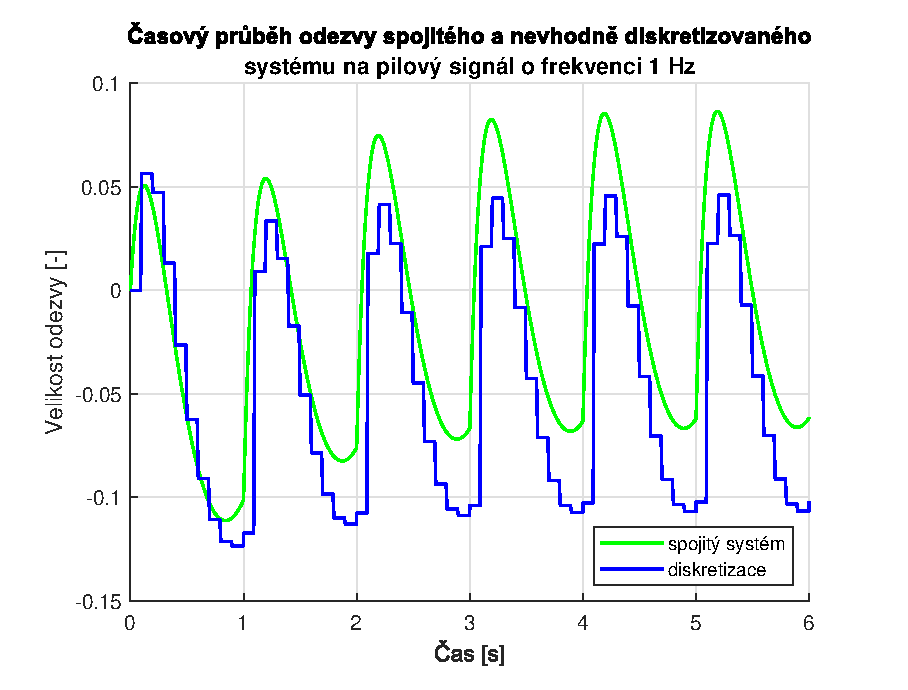
\includegraphics[width=\linewidth]{diskretizace-bad.eps}
		\caption{Nevhodná diskretizace s krokem $T_2 = 100$ ms}
	\end{subfigure}
	\caption{Srovnání odezvy vhodné a nevhodné diskretizace systému}
	\label{fig:diskretizace}
\end{figure}


Kdybychom přivedli na vstup signál s vyšší frekvencí, porušili bychom vzorkovací teorém a výstup diskretizací by byl podstatně odlišný od výstupu spojitého systému.
Diskretizace $G_1(z)$ díky desetkrát menšímu kroku má desetkrát větší šířku pásma a tudíž by byla spolehlivá o dekádu frekvencí déle než diskretizace $G_2(z)$.
Od frekvence $0.5 \cdot T_1^{-1} = 50$ Hz ale i vhodná diskretizace rychle akumuluje chybu a má jen málo společného se vstupním signálem či výstupem spojitého systému.
Toto chování je vidět na obrázku \ref{fig:diskretizace-rip}. To však není chyba diskretizace samotné, je to naše chyba, že jsme nedodrželi vzorkovací teorém.
\begin{figure}
	\centering
	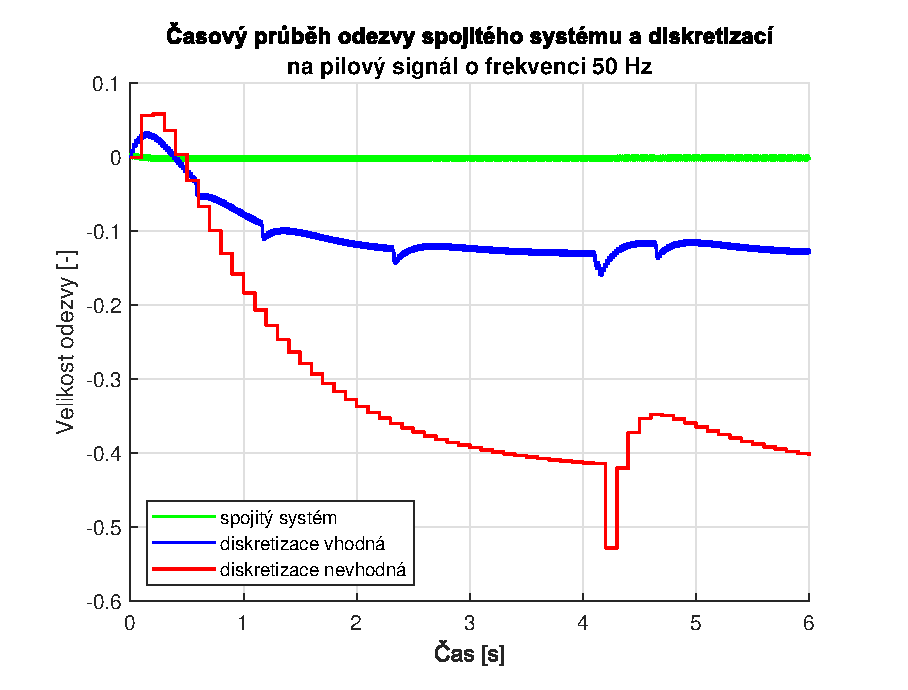
\includegraphics{diskretizace-rip.eps}
	\caption{Srovnání odezev spojitého systému a diskretizací při nedodržení vzorkovaních teorému}
	\label{fig:diskretizace-rip}
\end{figure}


\section{Vlastnosti přenosů}
\label{sec:ukol8}
Rozhodněte u každého z následujích přenosů, zdali jím popsaný systém je: stabilní/nestabilní, statický/astatický, kmitavý/nekmitavý.
\begin{equation*}
	\begin{split}
		G_1(s) &= -\frac{s-12}{(s+1)(5s+2)(s+3)} = -\frac{1}{5}~\frac{s-12}{(s+1)(s+0.4)(s+3)} \\
		G_2(s) &= \frac{1}{s^2 + 0.5s - 1} = \frac{1}{(s-0.7808)(s+1.2808)} \\
		G_3(s) &= \frac{1}{s^2} \\
		G_4(s) &= \frac{s+2}{s^2-2} = \frac{s+2}{(s-\sqrt{2})(s+\sqrt{2})}
	\end{split}
\end{equation*}

Vlastnosti budu vyčítat zejména z pólů přenosových funkcí, proto jsme rovnou rozložili polynomy na kořenové činitele.

\begin{itemize}
	\item \textbf{Stabilita}: Stabilní systém má reálnou složku všech pólů zápornou. Toto kritérium splňuje pouze systém s přenosem $G_1(s)$,
	ostatní mají alespoň jeden pól na imaginární ose nebo vlevo od ní.
	\item \textbf{Astatismus}: Astatický systém má integrační charakter, jeho chování je závislé na předchozím stavu. Přenos astatického 
	systému obsahuje alespoň jeden pól v počátku. Astatický je jen systém s přenosem $G_3(s)$, ostatní jsou statické.
	\item \textbf{Kmitání}: Systém s komplexně sdruženými póly bude kmitat, protože se do jeho impulsové charakteristiky promítnou goniometrické funkce
	(reálná a imaginární složka komplexní exponeniciály). Všechny zadané systémy ale mají póly reálné a tudíž kmitání nemůže nastat.
\end{itemize}






















\section{Spojování dynamických systémů}
\label{sec:ukol9}
Jsou dány dva systémy
\begin{equation*}
	G_1(s) = \frac{s-1}{s+1}, G_2(s) = \frac{1}{s}
\end{equation*}
odvoďte výsledný přenost $H(s)$ pro jejich různá zapojení. Zapojení (c) a (d) jsou ilustrována na \ref{fig:zapojeni}.
\begin{figure}[htbp]
	\centering
	\begin{subfigure}{0.45\textwidth}	
		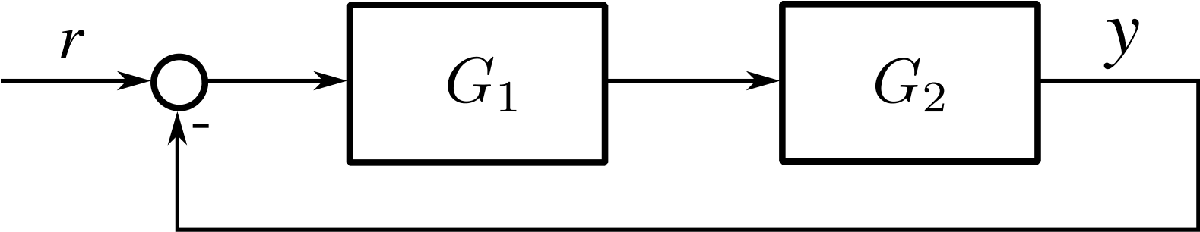
\includegraphics[width=.45\textwidth]{zadani9-3.png}
		\caption{Zapojení pro úlohu 9.3}
		\label{fig:zadani9-3}
	\end{subfigure}
	\begin{subfigure}{0.45\textwidth}
		\centering
		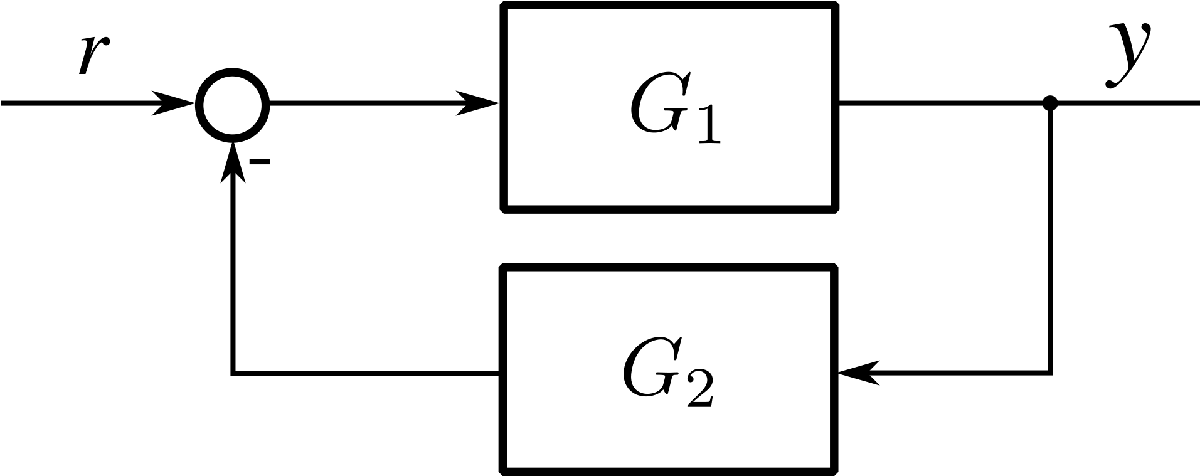
\includegraphics[width=.45\textwidth]{zadani9-4.png}
		\caption{Zapojení pro úlohu 9.4}
		\label{fig:zadani9-4}
	\end{subfigure}
	\caption{Ilustrace zapojení v úlohách 9.3 a 9.4}
	\label{fig:zapojeni}
\end{figure}
\subsection{Paralelní zapojení} 
\textbf{Řešení:} Paralelní zapojení systémů vede na prostý součet jejich přenosů. Proto je celkový přenos zapojení roven
\begin{equation*}
	H(s) = G_1(s) + G_2(s) = \frac{s-1}{s+1} + \frac{1}{s} = \frac{s(s-1) + (s+1)}{s(s+1)} = \frac{s^2 + 1}{s (s+1)}
\end{equation*}
\subsection{Kaskádní spojení}
\label{sec:ukol9:2}
\textbf{Řešení:} Kaskádní spojení vede na konvoluci v časové oblasti a násobení přenosů v oblasti obrazové. Proto je celkový přenos zapojení roven
\begin{equation*}
	H(s) = G_1(s) \cdot G_2(s) = \frac{s-1}{s(s+1)}
\end{equation*}
\subsection{Záporná zpětná vazba } 
\label{sec:ukol9:3}
Zpětnovazební spojení se zápornou zpětnou vazbou, kde přenosy G1 a G2 jsou v přímé vazbě (viz obr \ref{fig:zadani9-3}) \\
\textbf{Řešení:} Označme přenos kaskádního zapojení $G_1(s)$, $G_2(s)$ jako $G(s) = G_1(s)G_2(s) = \frac{s-1}{s(s+1)}$ (podle \ref{sec:ukol9:2}).
Tím se systém zjednodušil na jediný systém zapojený v dopředné cestě zpětnovazební smyčky. Označíme-li $x(s)$ signál za sčítačkou, poté platí
\begin{equation*}
	y(s) = G(s) \cdot x(s) = G(s) \cdot (r(s) - y(s)) \Rightarrow y(s) (1 + G(s)) = G(s) \cdot r(s).
\end{equation*}
Celkový přenos systému je
\begin{equation*}
	H(s) = \frac{y(s)}{r(s)} = \frac{G(s)}{1 + G(s)} = \frac{s^3 - s}{s^4 + 3s^3 + s^2 - s} = \frac{s(s-1)(s+1)}{s(s+1)(s-0.4142)(s+2.4142)}.
\end{equation*}
\subsection{Záporná zpětná vazba } 
Zpětnovazební spojení se zápornou zpětnou vazbou s G1 v přímé vazbě a G2 ve zpětné vazbě (viz obr \ref{fig:zadani9-4}) \\
\textbf{Řešení:} Podobně jako \ref{sec:ukol9:3} popíši systém rovnicemi. Označme $x(s)$ signál na výstupu sčítačky. Podle schématu platí:
\begin{equation*}
	y(s) = G_1(s) \cdot x(s) = G_1(s) \cdot (r(s) - G_2(s) \cdot y(s)) \Rightarrow y(s) (1 + G_1(s)G_2(s)) = G_1(s) \cdot r(s).
\end{equation*}
Celkový přenos systému je
\begin{equation*}
	H(s) = \frac{y(s)}{r(s)} = \frac{G_1(s)}{1 + G_1(s)G_2(s)} = \frac{s^3 - s}{s^3 + 3s^2 +s - 1} = \frac{s(s-1)(s+1)}{(s+1)(s-0.4142)(s+2.4142)}.
\end{equation*}
\section{Diskrétní systém}
\label{sec:ukol10}
Je zadán diskrétní systém
\begin{equation}
	\label{eq:diferencni}
	3y(k) - y(k-1) + 0.5 y(k-2) = u(k-1)-u(k-2)
\end{equation}

\subsection{~}
Vyjádřete přenos systému. \\
\textbf{Řešení:} Použiji Z-transformaci diferenční rovnice popisující systém. Nechť $Y(z) = \mathcal{Z}\{y(k)\}$ a $U(z) = \mathcal{Z}\{u(k)\}$, poté \eqref{eq:diferencni} upravíme na
\begin{equation}
	\begin{split}
		3Y(z) - z^{-1} Y(z) + 0.5 z^{-2} Y(z) &= z^{-1}U(z) - z^{-2}U(z) \\
		Y(z) (3- z^{-1} + 0.5 z^{-2}) &= U(z) (z^{-1} - z^{-2}) \\
		H(z) = \frac{Y(z)}{U(z)} &= \frac{z^{-1} - z^{-2}}{3-z^{-1}+ 0.5z^{-2}}, ~~~~\text{rozšiřme členem $z^2$} \\
		H(z) &= \frac{z - 1}{3z^2-z+ 0.5}.
	\end{split}
\end{equation}

\subsection{~}
Rozhodněte o stabilitě systému. Rozhodnutí zdůvodněte. \\
\textbf{Řešení:} Přenosová funkce má dva komplexně sdružené póly $ z_{1,2} = 0.1667 \pm 0.3727i$. Aby byl stabilní, musí ležet póly uvnitř jednotkové kružnice v z-rovině.
Tento požadavek je zde zřejmě splněn, protože $\vert z_{1,2} \vert < 1 $ a systém je tedy stabiltní.
\subsection{~}
Nakreslete simulinkové schéma realizace tohoto přenosu pro vstup u a výstup y a vykreslete jeho odezvu
na jednotkový skok pro vzorkovací periodu h = 1. \\
\begin{figure}
	\centering
	\includegraphics[height=14cm]{diskretni_system.pdf}
	\caption{Schéma diskrétního systému pro úlohu 10}
	\label{fig:diskretni_schema}
\end{figure}
\textbf{Řešení:} Schéma systému je na obrázku \ref{fig:diskretni_schema}, výstup simulace odezvy poté na obrázku \ref{fig:odezva_step}.
\begin{figure}
	\centering
	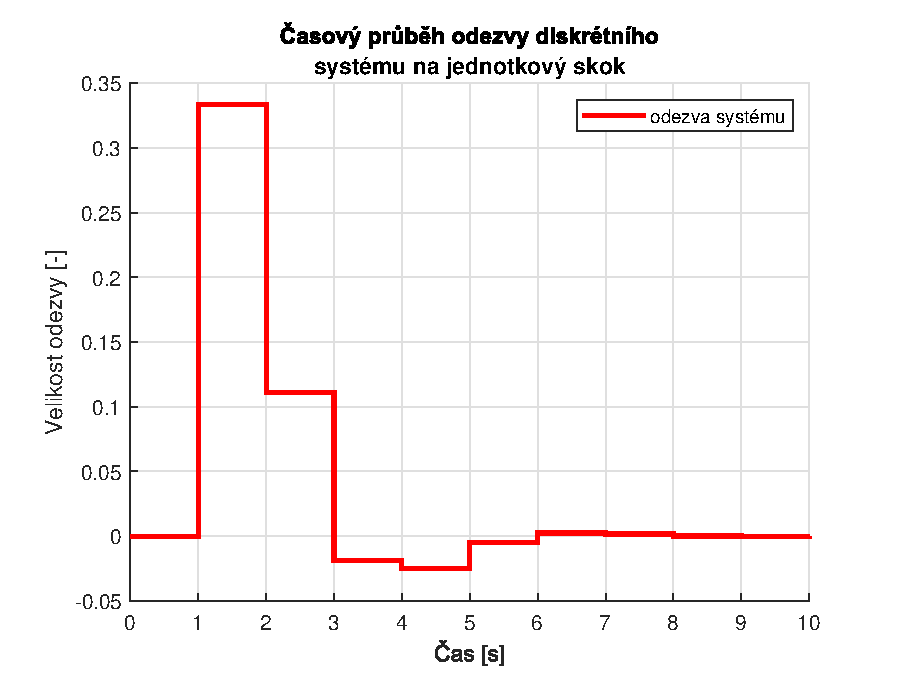
\includegraphics[height=9cm]{discrete_response_step.eps}
	\caption{Odezva diskrétního systému z úlohy 10 na jednotkový skok}
	\label{fig:odezva_step}
\end{figure}

\newpage

\section{ Skokové (přechodové) a impulzní charakteristiky}
\label{sec:ukol11}
Na obrázku \ref{fig:charakteristiky} jsou zobrazeny tři impulzní a tři přechodové charakteristiky pro tři různé systémy.

\subsection{~}
Přiřaďte správně skokové charakteristiky impulzním charakteristikám tak, aby odpovídaly stejnému systému. \\
\textbf{Řešení:} Podle vztahu popsaného v \ref{sec:ukol11:2} lze k sobě přiřadit odezvy podle tabulky \ref{tab:odezvy}.
\begin{table}[htbp]
	\centering
	\begin{tabular}{c|c|c}
		$h(t)$ & $w(t)$ & poznámka \\
		\hline
		c & e & integrál konstantní $h(t) \neq 0 $ roste lineárně a diverguje \\
		b & d & $h(t)$ i $w(t)$ exponeniciální průběh \\
		a & f & $h(t)$ kmitá, kmity nalézáme i na $w(t)$
	\end{tabular}
	\caption{Přiřazení odezvy na Diracův impuls a na jednotkový skok}
	\label{tab:odezvy}
\end{table} 

\subsection{~}
\label{sec:ukol11:2}
Jaký obecně mezi sebou mají impulzní charakteristika $h(t)$ a skoková charakteristika $w(t)$ vztah? \\
Řešení (viz \ref{sec:ukol1:3}): Protože spojitý lineární systém zachovává vztahy jako integrál a derivace,
je vztah $h(t)$ a $w(t)$ stejný jako vztah signálů $\delta(t)$ a $\mathbb{1}$(t). Platí
\begin{equation*}
	h(t) = \frac{\dif}{\dif t} w(t) ~~~~~~~~~ a ~~~~~~~~~ w(t) = \int_{-\infty}^{t} h(\tau) \dif \tau.
\end{equation*}


\begin{figure}[htbp]
    \centering % <-- added
\begin{subfigure}{0.25\textwidth}
  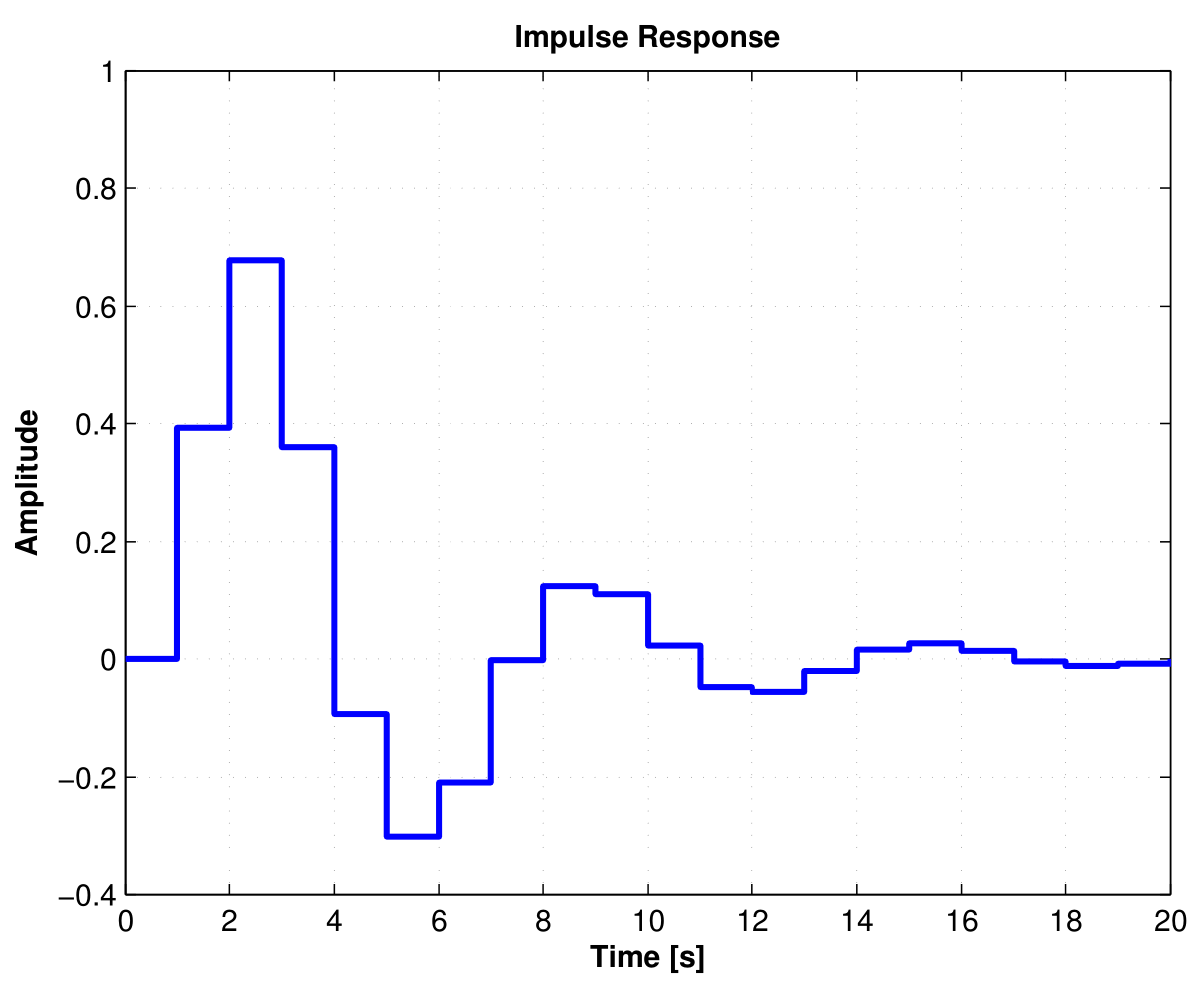
\includegraphics[width=\linewidth]{zadani11-a}
  \caption{}
  \label{fig:charakteristiky:a}
\end{subfigure}\hfil % <-- added
\begin{subfigure}{0.25\textwidth}
	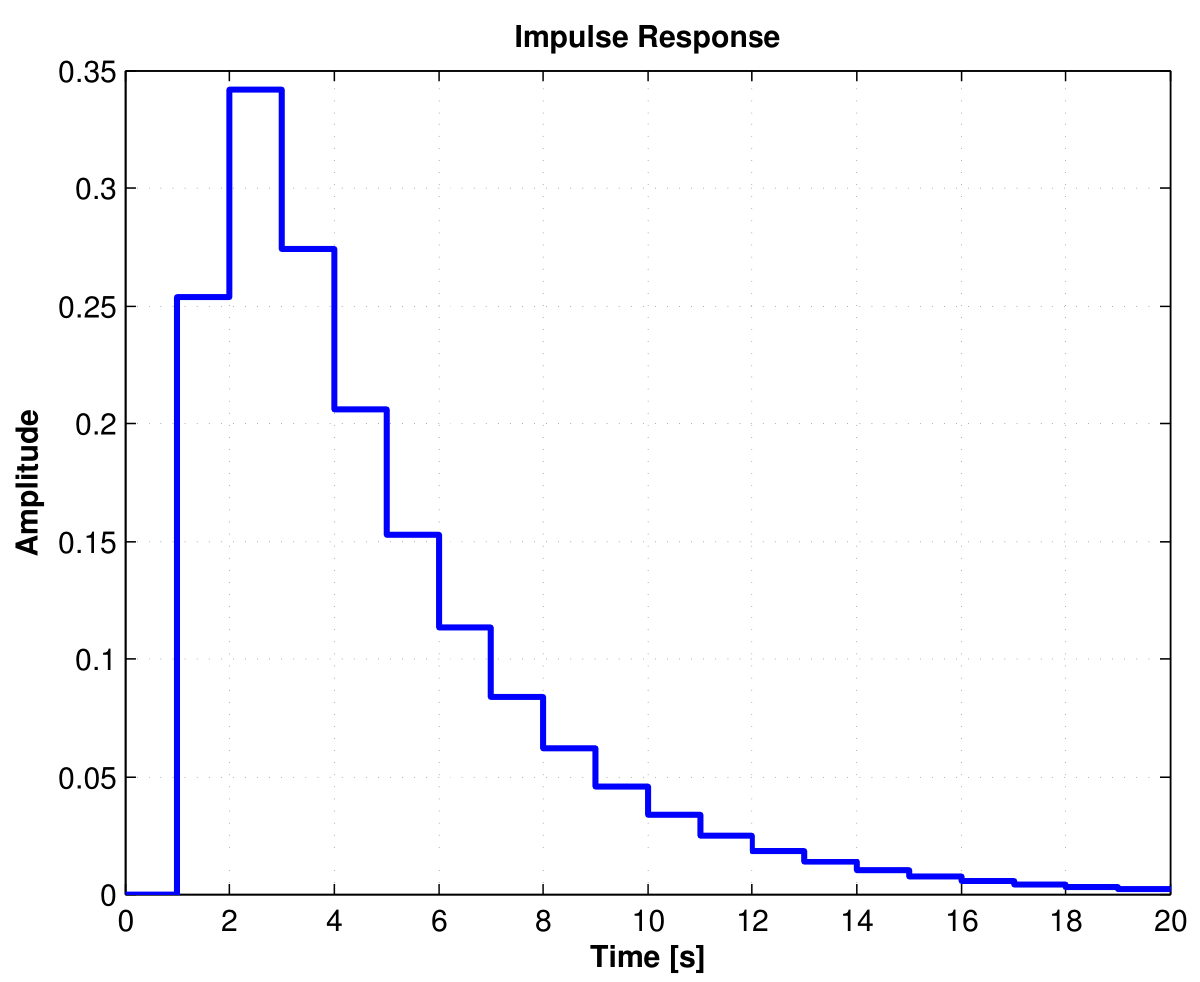
\includegraphics[width=\linewidth]{zadani11-b}
	\caption{}
	\label{fig:charakteristiky:b}
\end{subfigure}\hfil % <-- added
\begin{subfigure}{0.25\textwidth}
	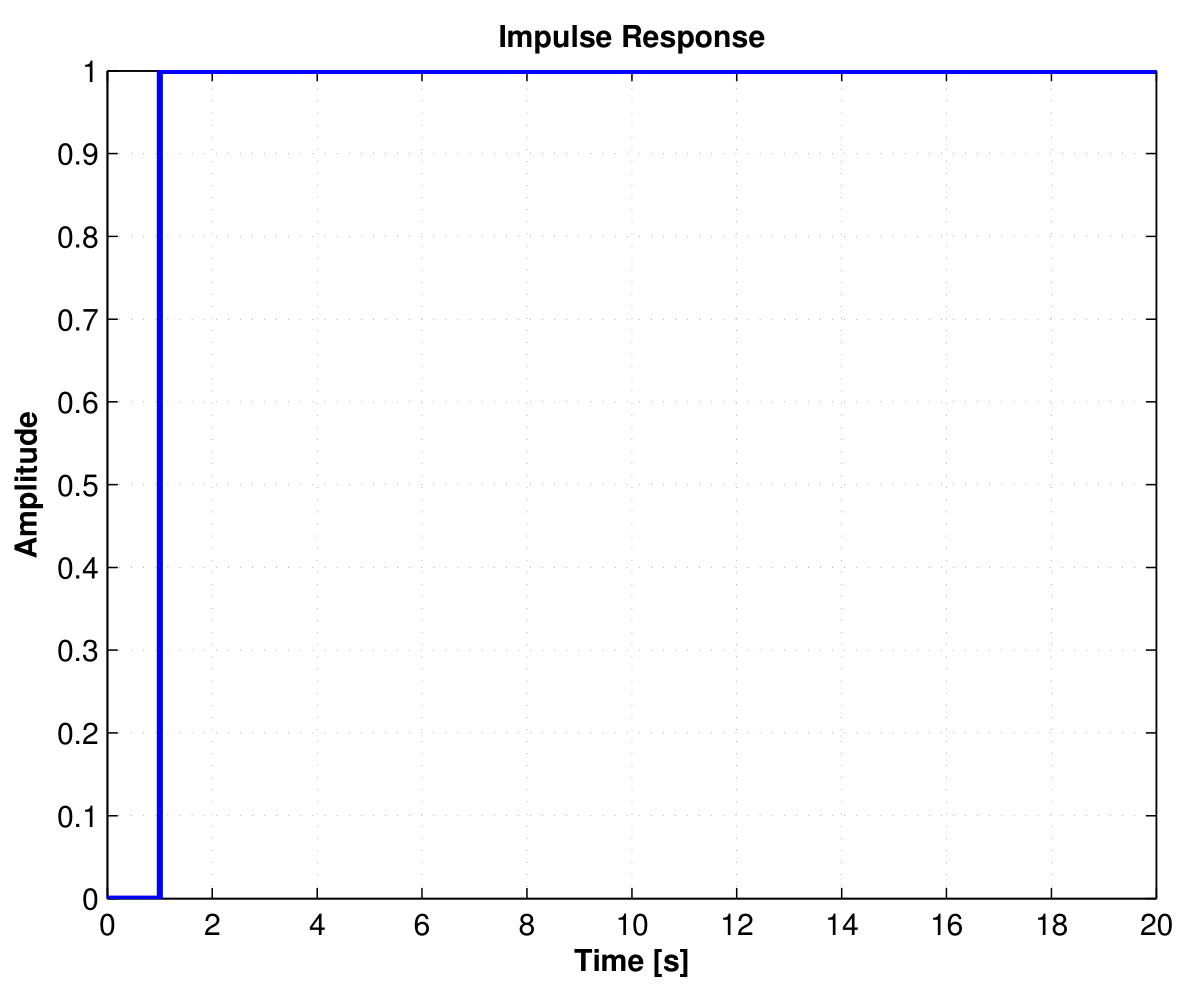
\includegraphics[width=\linewidth]{zadani11-c}
	\caption{}
  \label{fig:charakteristiky:c}
\end{subfigure}

\medskip
\begin{subfigure}{0.25\textwidth}
  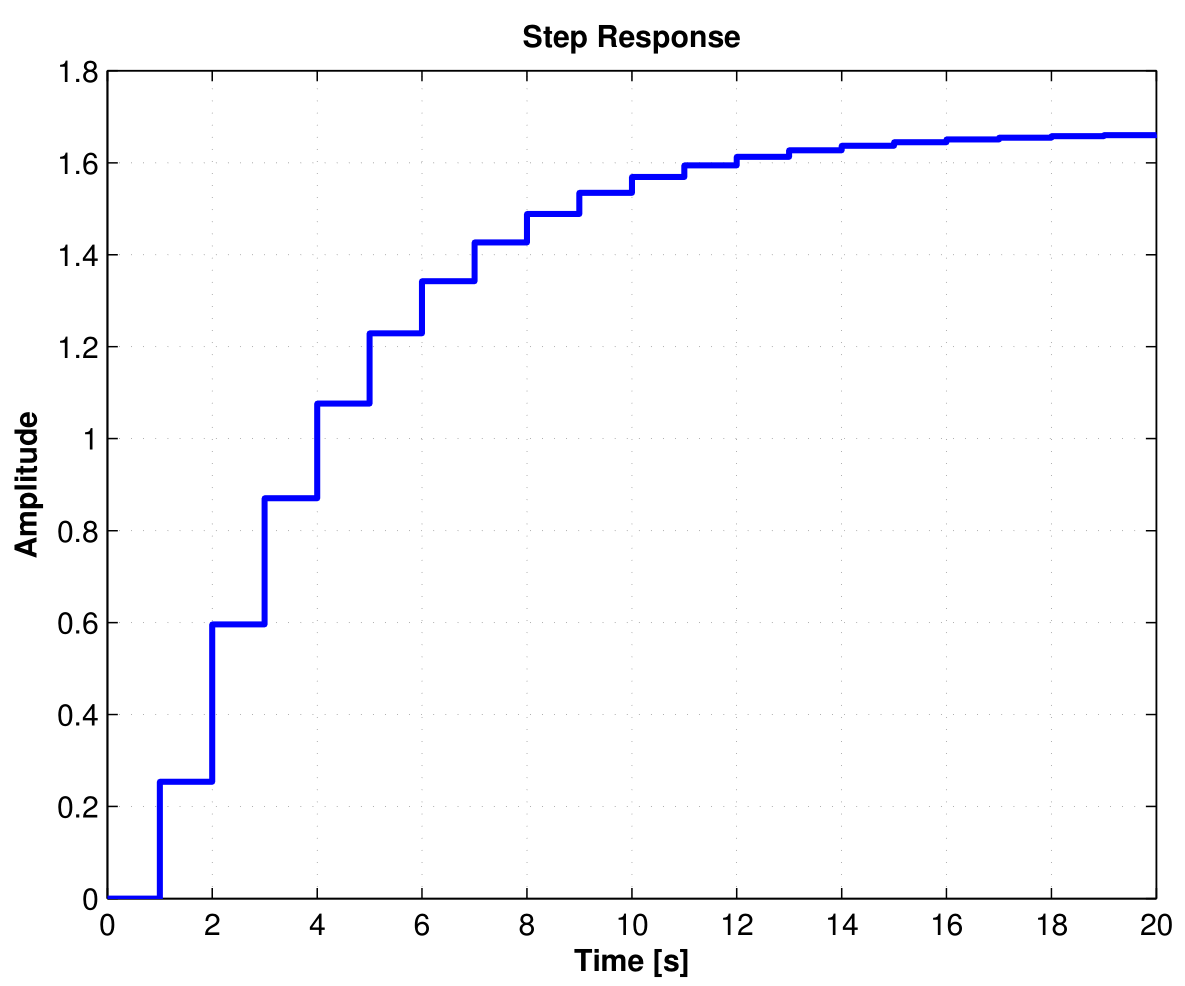
\includegraphics[width=\linewidth]{zadani11-d}
  \caption{}
  \label{fig:charakteristiky:d}
\end{subfigure}\hfil % <-- added
\begin{subfigure}{0.25\textwidth}
	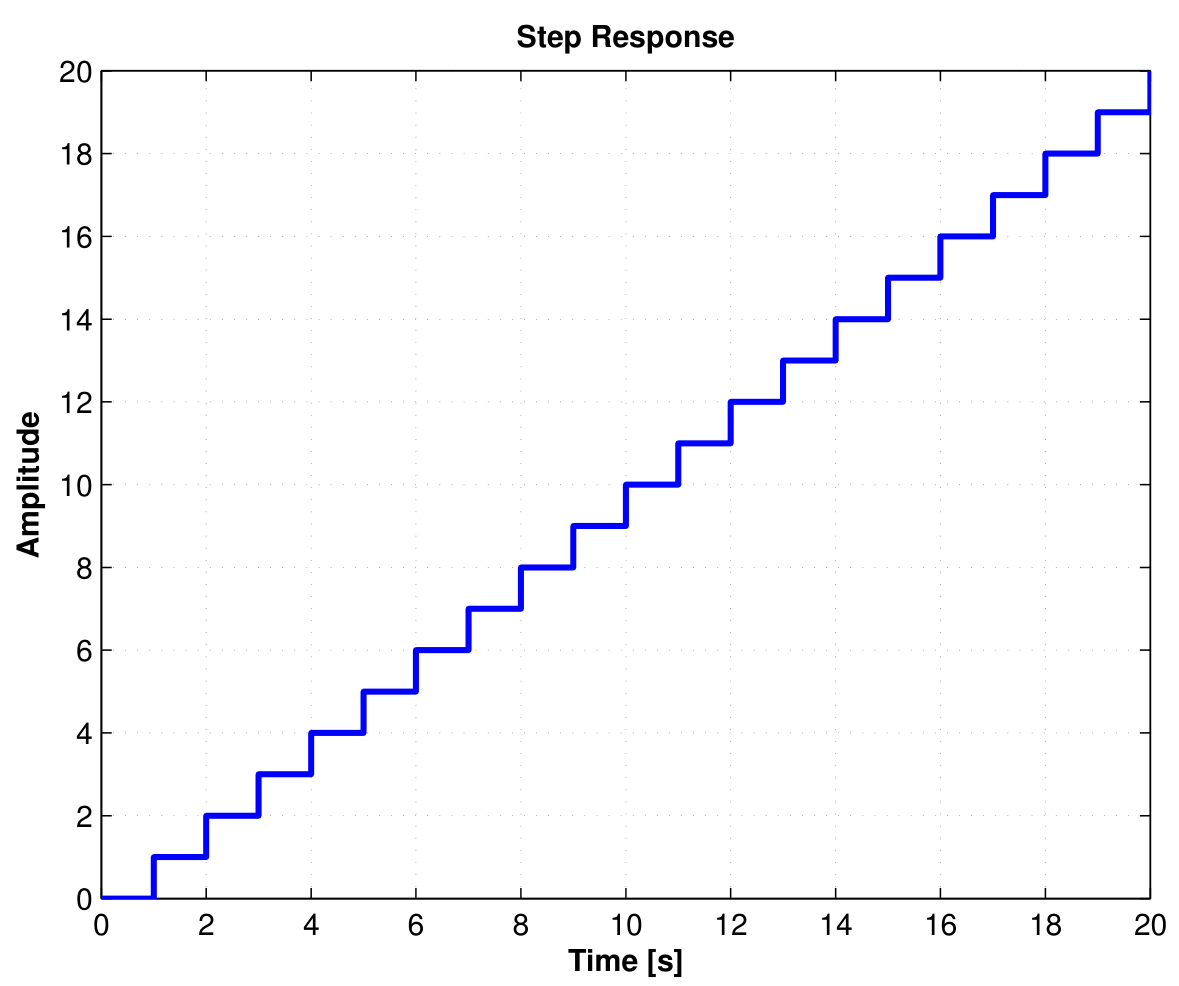
\includegraphics[width=\linewidth]{zadani11-e}
	\caption{}
	\label{fig:charakteristiky:e}
\end{subfigure}\hfil % <-- added
\begin{subfigure}{0.25\textwidth}
	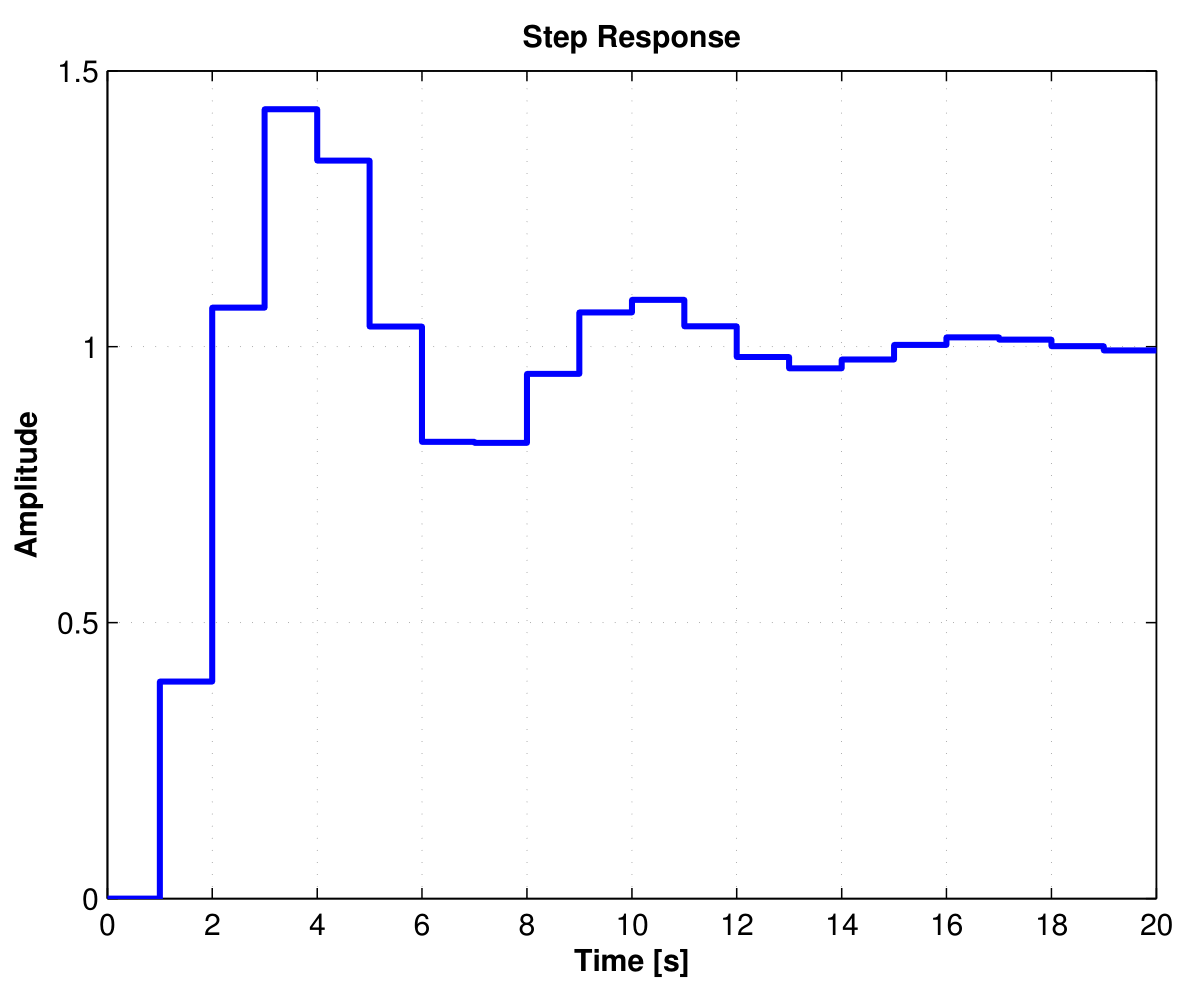
\includegraphics[width=\linewidth]{zadani11-f}
  \label{fig:charakteristiky:f}
  \caption{}
\end{subfigure}
\caption{Charakteristiky k identifikaci}
\label{fig:charakteristiky}
\end{figure}

\newpage

\section{Frekvenční charakteristiky}
\label{sec:ukol12}
Na obrázku \ref{fig:frekchar} jsou zobrazeny Bodeho frekvenční charakteristiky a Nyquistovy frekvenční charakteristiky tří systémů.
\subsection{~}
Přiřaďte k sobě frekvenční charakteristiky odpovidající stejnému systému. \\
\textbf{Řešení:} Při přiřazení charakteristik si musím vystačit s obecným trendem fáze a amplitudy, protože z Nyquistovy char. nelze odečíst přesná frekvence.
Amplitudy v této úloze nebyly příliš nápomocné, všechny charakteristiky lze určit pohledem na fáze. Jedna dvojice má fáze konstantní,
druhá dvojice mění fázi na celém spektru jen o 90° a poslední o 270°.
Charakteristiky lze přiřadit podle tabulky \ref{tab:charakteristiky}.
\begin{table}[htbp]
	\centering
	\begin{tabular}{c|c|c}
		Bode & Nyquist & poznámka \\
		\hline
		c & e & jediná možnost s konstantní fází, amplitudy omezeny shora \\
		a & f & pro $\omega \rightarrow 0$ je fáze 0, celkem změna fáze -90° \\
		b & d & celkem změna fáze o 270°
	\end{tabular}
	\caption{Přiřazení odpovídajících si frekvenčních charakteristik}
	\label{tab:charakteristiky}
\end{table}
\subsection{~}
U frekvenční charakteristiky na obrázku \ref{fig:frekchar:f} najděte pro fázi -45° zesílení systému (v dB). \\
\textbf{Řešení:} Komplexní čísla $z$ s fází -45° leží na přímce s předpisem $ \Re(z) = - \Im(z)$. Jejím průsečíkem s danou Nyquistovou charakteristikkou
je bod $z_0 = 0.5 - 0.5i$. Zesílení systému v daném bodě charakteristiky je 
\begin{equation}
	\abs{z} = \sqrt{\frac{2}{4}} = \frac{1}{\sqrt{2}},
\end{equation}
což v logaritmických souřadnicích odpovídá zesílení $20 \log{\frac{1}{\sqrt{2}}} = -3$ dB.


\begin{figure}[htbp]
    \centering % <-- added
\begin{subfigure}{0.25\textwidth}
  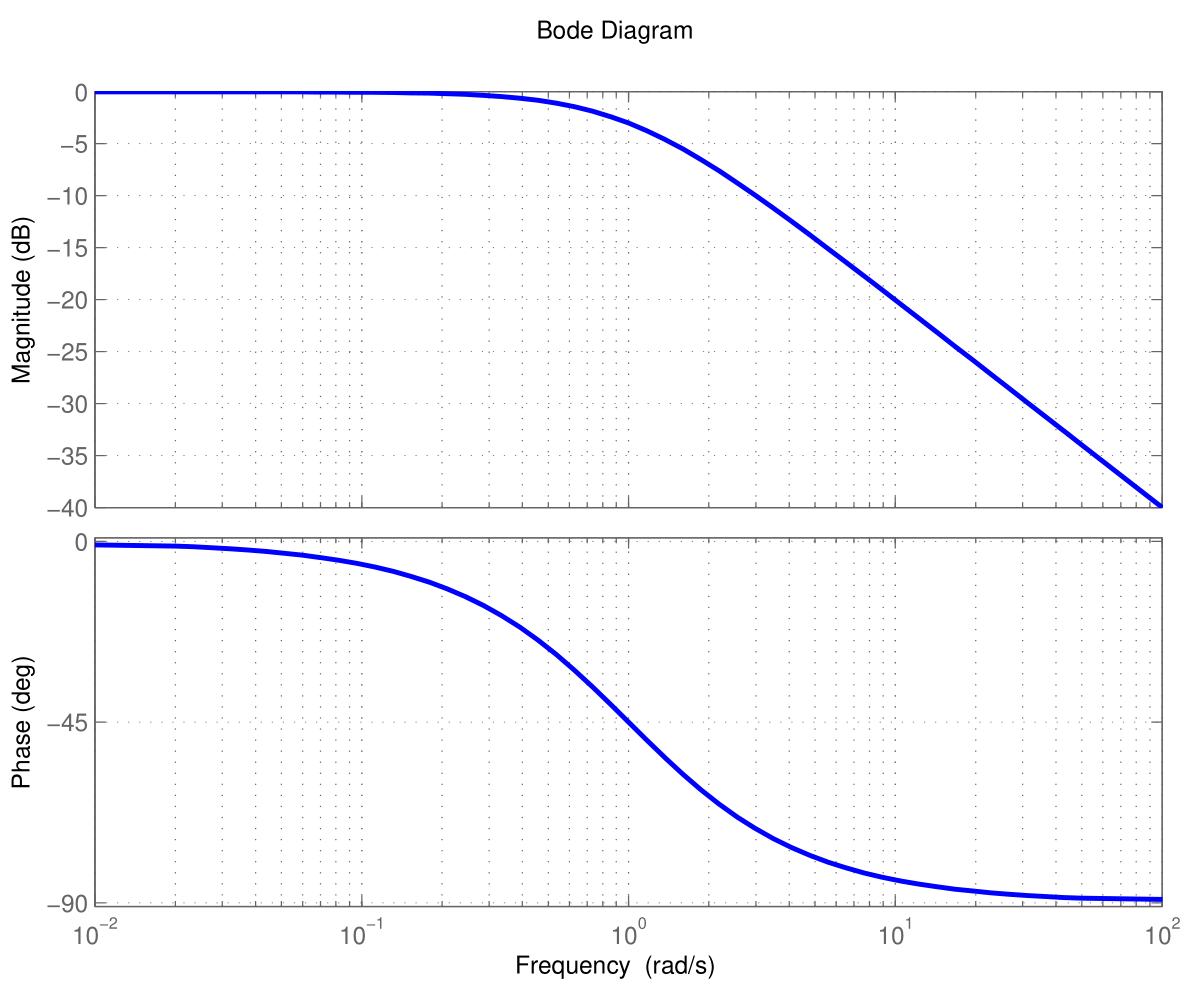
\includegraphics[width=\linewidth]{zadani12-a}
  \caption{}
  \label{fig:frekchar:a}
\end{subfigure}\hfil % <-- added
\begin{subfigure}{0.25\textwidth}
	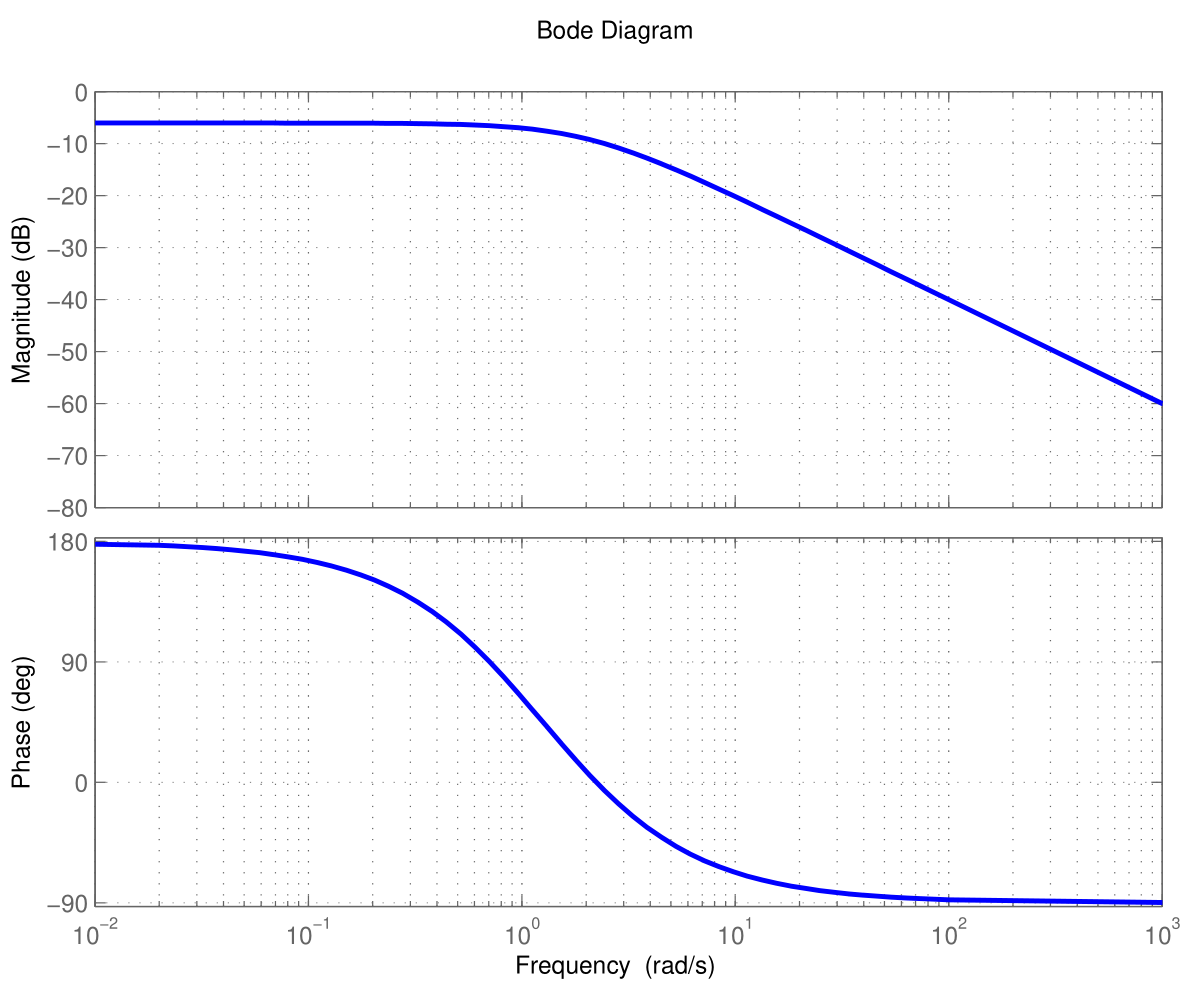
\includegraphics[width=\linewidth]{zadani12-b}
	\caption{}
	\label{fig:frekchar:b}
\end{subfigure}\hfil % <-- added
\begin{subfigure}{0.25\textwidth}
	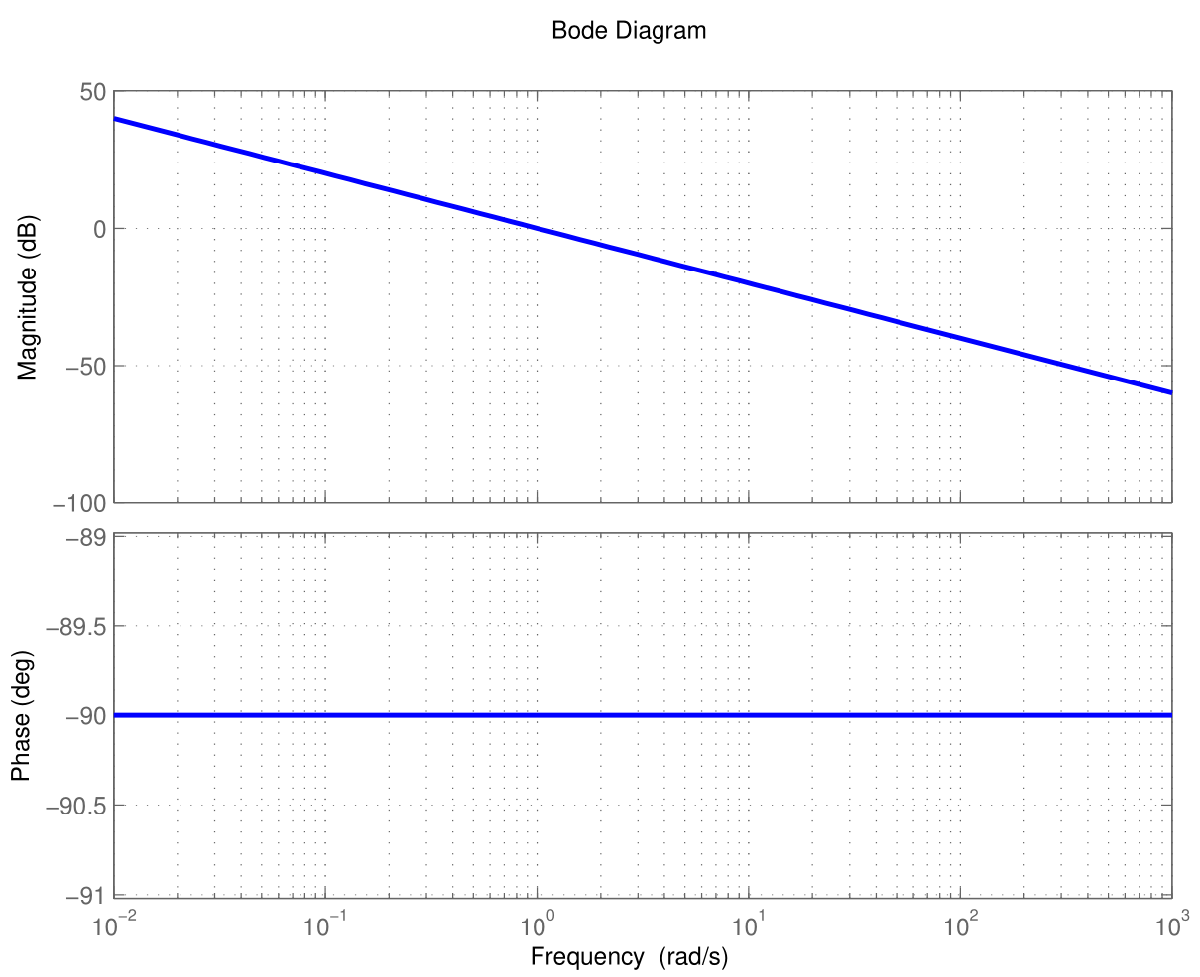
\includegraphics[width=\linewidth]{zadani12-c}
  \caption{}
  \label{fig:frekchar:c}
\end{subfigure}

\medskip
\begin{subfigure}{0.25\textwidth}
  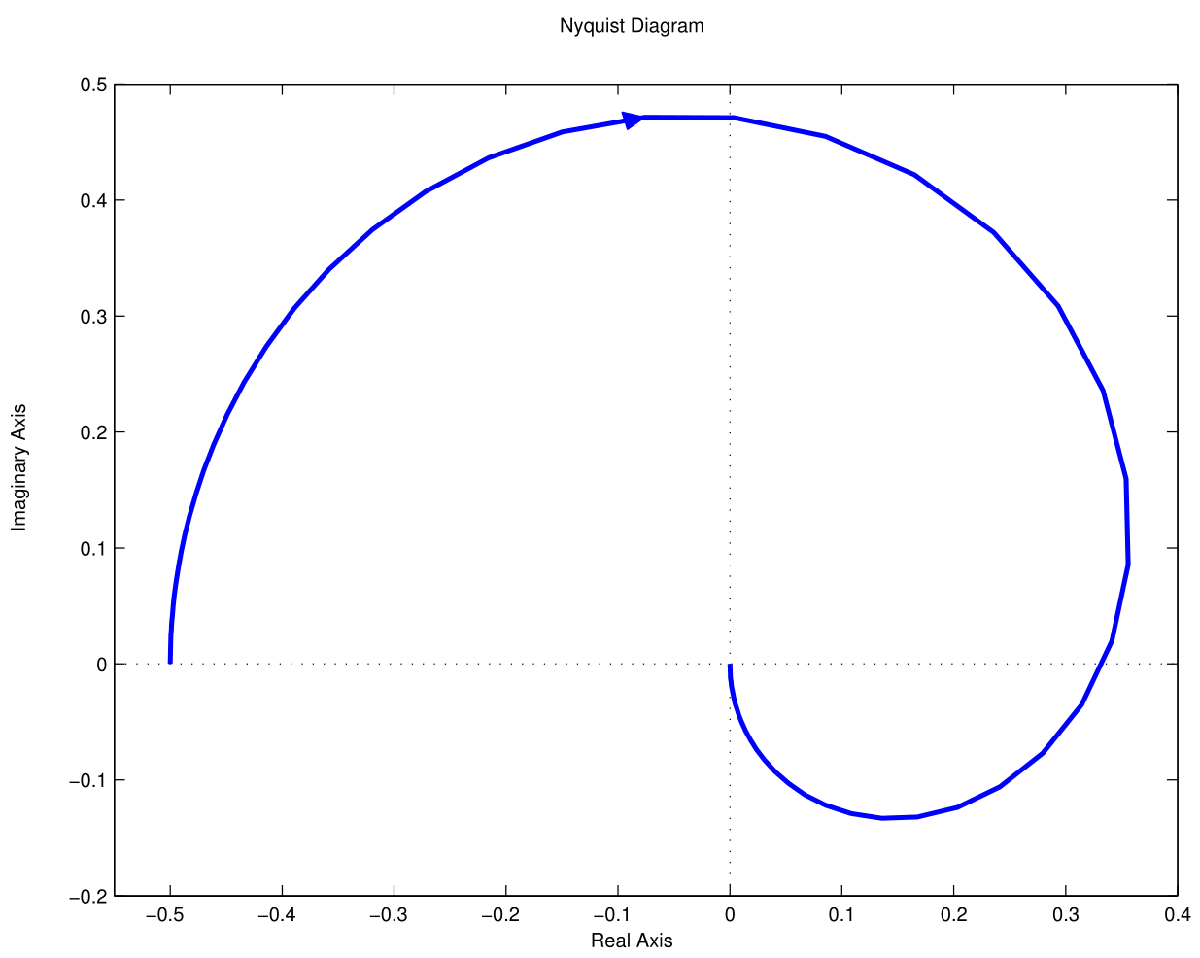
\includegraphics[width=\linewidth]{zadani12-d}
  \caption{}
  \label{fig:frekchar:d}
\end{subfigure}\hfil % <-- added
\begin{subfigure}{0.25\textwidth}
	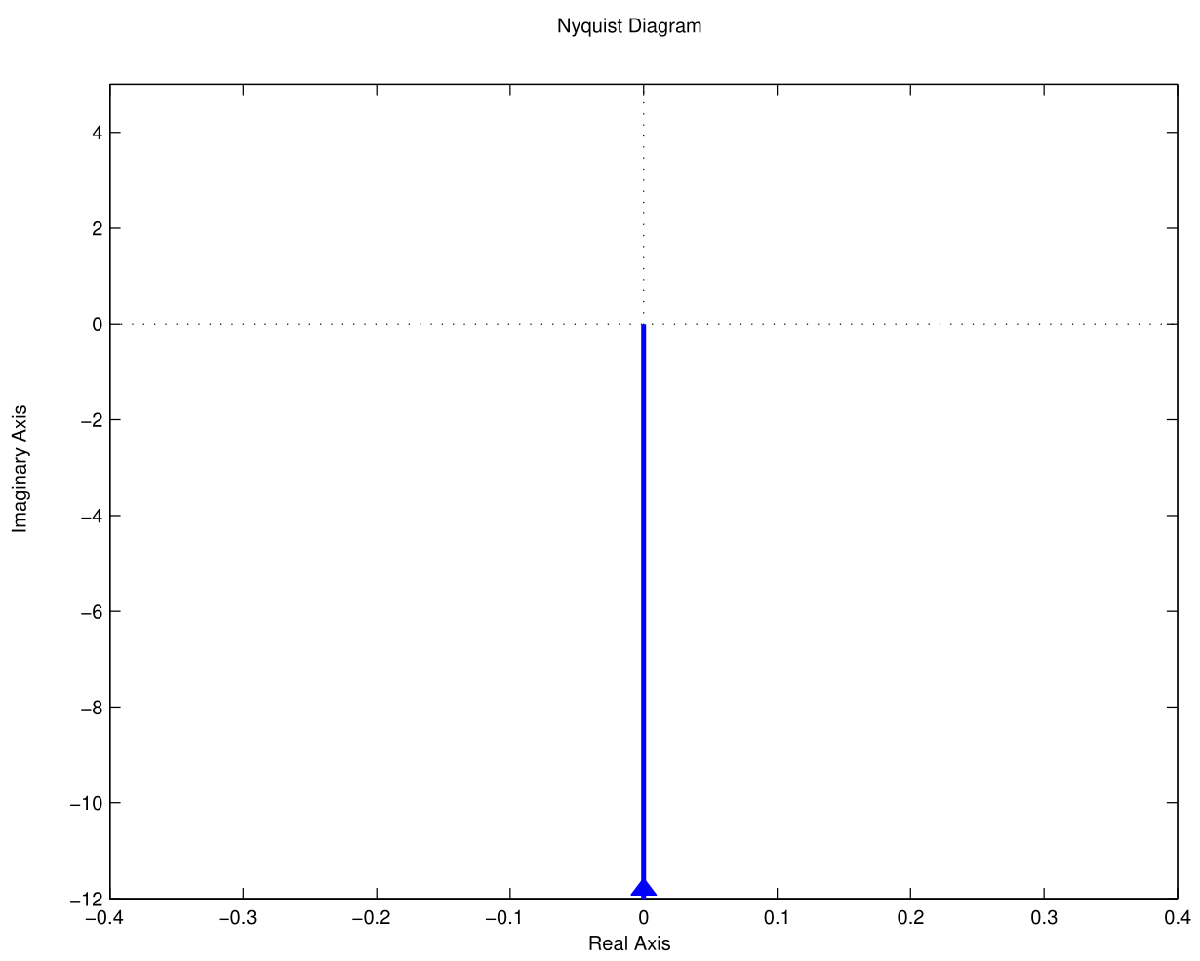
\includegraphics[width=\linewidth]{zadani12-e}
	\caption{}
	\label{fig:frekchar:e}
\end{subfigure}\hfil % <-- added
\begin{subfigure}{0.25\textwidth}
	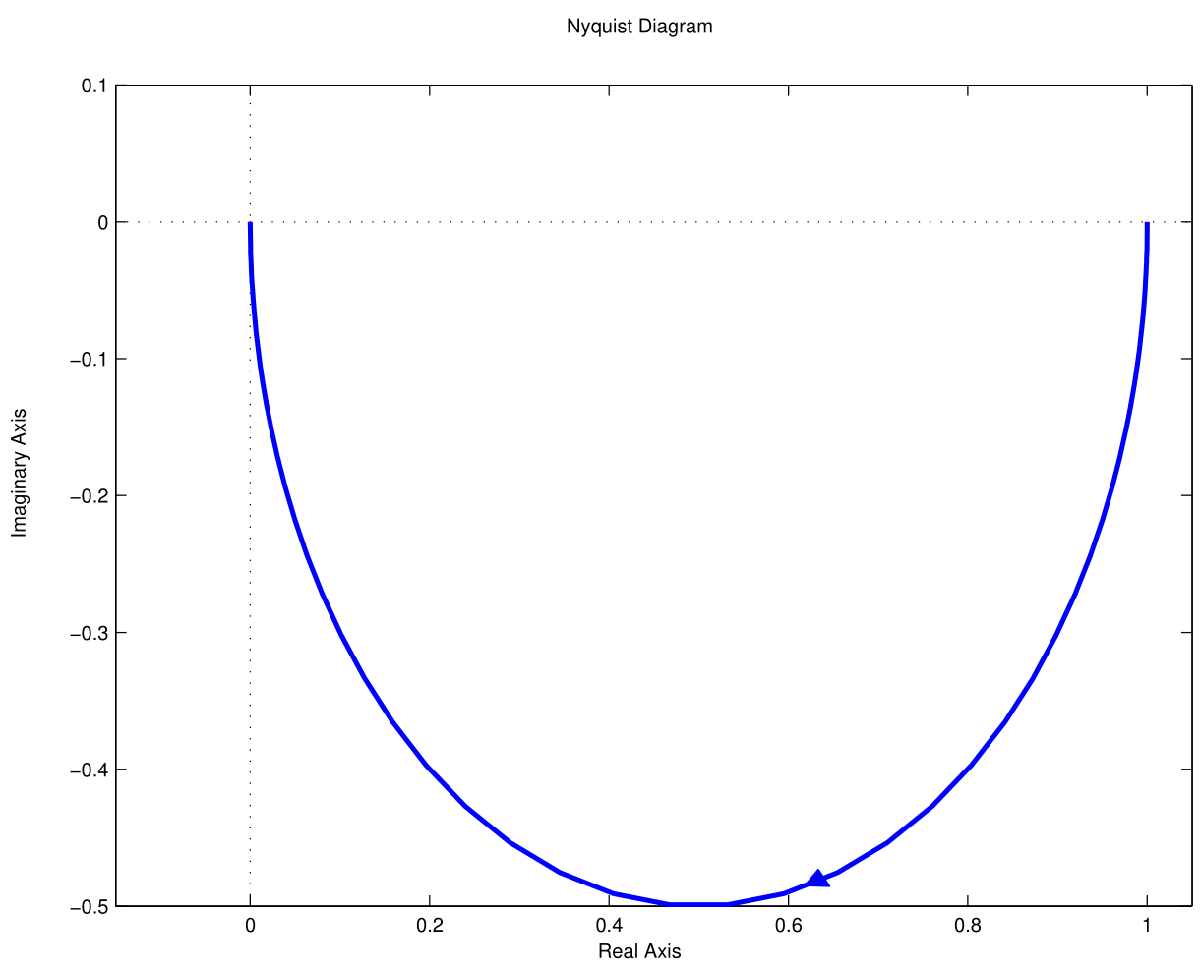
\includegraphics[width=\linewidth]{zadani12-f}
  \caption{}
  \label{fig:frekchar:f}
\end{subfigure}
\caption{Frekvenční charakteristiky ke spojení}
\label{fig:frekchar}
\end{figure}




% ---------------------------------
% ---------------------------------
% Literatura
\begin{thebibliography}{9}


\bibitem{Wiki}
	\LaTeX tutorials, \url{http://en.wikibooks.org/wiki/LaTeX/}

\bibitem{motivace}
	Motivační hudba, \emph{Kirby dream land theme song} \url{https://www.youtube.com/watch?v=3CS93CdMv_E}

\end{thebibliography}












\end{document}

